\chapter[BDM's EUM as ABM]{BDM's EUM as ABM: Agentizing the Expected Utility Model}

\section{Introduction}

In a series of papers and books across several decades, Bruce Bueno de Mesquita (commonly referred to as BDM) has presented and applied several versions of a forecasting model to predicting everything from internal Iranian power struggles \citeyearpar{bdm_1984} and European regulation negotiations \citeyearpar{bdm_1994} to the course of the entire Cold War \citeyearpar{bdm_1998}. The model is intended to simulate the iterative negotiation process between multiple actors, identifying where they compromise and where they attempt to coerce one another. It has attracted widespread attention (particularly by the standards of political science models): it was the subject of a special journal issue \citep{kugler_1997}, and was featured in a popular-audience TED talk \citep{bdm_2009} and book \citep{bdm_2010}. It can be used not only for prediction but also decision support \citep{root_2013}, and has reportedly been successfully applied by the Central Intelligence Agency \citep{feder_1992}, as well as numerous commercial clients of Decision Insights, Incorporated (a consulting firm BDM co-founded). The model was even the subject of a lawsuit by that company against a rival \citep{dii_2011} accused of stealing the model. 

Such a universal political forecasting model is worth examining in detail. BDM and his collaborators have described the model extensively \citep{bdm_1984,bdm_1994,bdm_1997,bdm_2002,bdm_2011}, but have never published the full specifications, and in particular never made the underlying code available. Several attempts have been made to replicate it from published material \citep{scholz_2011,kimbrough_2014,mckibben_sanders_2014}, but none of these have successfully fully reproduced its reported results. Indeed, as \citet{scholz_2011} document, some details of the model appear to have changed over time\footnote{These changes suggest that there is not a single `original' model to reproduce. Nevertheless, as BDM does not clearly demarcate different generations or variants, I will use phrase `original model' in this chapter to refer to my overall understanding of the model. My own implementation primarily followed the description provided in \citet{bdm_2002}.}, and testimony in the \citet{dii_2011} lawsuit states that the commercial version of the model contains trade secrets not reproducible from the public literature. There have also been several attempts to develop similar models: these include an internal CIA variant \citep{feder_1992}; the Senturion toolkit \citep{abdollahian_2006} (the competitors' model which triggered the lawsuit mentioned above); at least one more proprietary model that I am aware of; and the \citet{wise_2015a} Toolkit for Behavioral Analysis. Of these, only the last is open source; the rest are proprietary commercial products.

BDM has characterized the model as grounded in micro-economics \citep{bdm_1994} and game theory \citep{bdm_2002,bdm_2009,bdm_2010}, and often refers to it as the Expected Utility Model (EUM) \citep{bdm_1984} -- borrowing a key term from game theory and economics. Indeed, the EUM bears many of the hallmarks of a formal model. \citet{scholz_2011} describes the model's underlying interactions as an extensive-form game tree. Several of the model's internal specifications closely resemble those used in the International Interaction Game (IIG) \citep{bdm_1992}, the game-theoretic model of international conflict described in the previous chapter, and \citet{bdm_2011} proposes an update to the model which directly incorporates the IIG's extensive-form tree as well. Yet despite the game-theoretic components, the model bears some clear differences from conventional game theory. It is intended to model and predict particular real-world interactions rather than to identify general patterns and theories \citep{snidal_1985}. None of the papers discussing the model have analyzed it in closed form to identify and parameterize its equilibria, and it is unclear whether such equilibria exist, or are meaningful. Indeed, the problem of identifying formal equilibria of games with more than two players becomes rapidly intractable \citep{papadimitriou_2005}. Thus, unlike in the majority of game theory models, the players are not assumed to be perfectly rational; they are explicitly boundedly-rational, using a variety of heuristics and looking at most one step ahead \citep{bdm_2002}. Finally, the model is implemented computationally, with the overall model, and each actor within it, executing set calculations and methods sequentially, and updating accordingly. While the model is largely described in terms of the specific calculations the agents make, I argue that these calculations are best viewed as particular sub-models rather than the model itself. In fact, another model, the \citet{stokman_1994} logrolling model, which takes the same inputs as the EUM and is intended for comparison with it, is explicitly described as an object-oriented computational model. Similarly, \citet{root_2013} also describe the model as agent-based. Understanding the model as an ABM emphasizes that the numeric calculations are not necessarily the most important components of it; the particular agent behavior rules, and the way the model sequences them, are equally important. Furthermore, treating the model as an ABM suggests additional methodological tools we can use to analyze it, such as sensitivity analyses and parameter sweeps \citep{gilbert_2005}.

Unlike the International Interaction Game presented in the previous chapter, the EUM cannot be viewed as a direct translation of a particular qualitative theory into model form. To be sure, several components of the model are grounded in specific theories. The definition, and significance, of the median voter position are drawn from the \citet{black_1948} economic analysis of collective decisionmaking; the risk propensity calculation, meanwhile, is adapted from Prospect Theory \citep{kahneman_1984} as detailed further in Section \ref{risk_update}. Beyond that, however, the model follows general assumptions from Realist theories -- the political actors are unitary entities, rationally maximizing their utility and cooperating only inasmuch as such cooperation is in their immediate interest -- but its details (such as the expected utility calculations and the offer-based interactions) cannot be traced to particular qualitative descriptions of state interactions, or political interactions more broadly. Put another way: the model is itself a theory of political interaction, competition and decisionmaking.

This chapter attempts to address several inter-connected questions and issues. The EUM has been utilized in multiple papers and developed a receptive audience, making it interesting to study and replicate, in order to test its accuracy independently, understand its driving assumptions, and potentially enable us to use it in future research. In the course of this replication, I argue that the model is best understood as an agent-based model, making it an important example of an ABM with predictive power and both academic and policy relevance. Such models are rare in general, and all the more so in the realm of international relations. Finally, I argue that the model can serve as the basis for comparative modeling of political conflicts. By using fixed inputs and modifying the assumptions and theories embedded in the model code, we can directly compare the effects implied by these theories, and test their explanatory and predictive power. If a model variant utilizing one theory produces more accurate outputs than one using a different theory, this is evidence that the theory is a better representation the system being modeled. Such comparison is particularly important given the model's numerous sub-models and weak grounding in prior theories, as it allows us to test whether the assumptions the sub-models make contribute to or detract from the model's overall explanatory and predictive power.

I have attempted to reimplement the Expected Utility model as an object-oriented, agent-based computer simulation. In this chapter, I restate the model following the ODD (Overview, Design concepts, Details) outline \citep{grimm_2006}, highlighting the entities, variables and sub-models from which the model is assembled (Section \ref{model_description}). I describe my attempt to validate the model against previous results (Section \ref{verification}) and conduct a deep dive into a single model step to describe and verify its behavior (Section \ref{deep-dive}). I then discuss the assumptions embedded in the model structure and implementation (Section \ref{bdm_discussion}), and propose several sub-model variations which can be easily swapped into the model implementation. In Section \ref{sensitivity-analysis}, I describe a sensitivity analysis I conduct using artificial input data sets. In Section \ref{info_extraction} I describe the output data the model generates, which can be compared to empirical data or used for prediction. Finally, In Section \ref{icews}, I apply the model in a novel way, implementing several of my proposed model variants and comparing their outputs to micro-level political event data.

\section{Model Description} \label{model_description}

The following section is written approximately following the ODD protocol \citep{grimm_2006}. I first provide an overview of the model (Section \ref{overview}), including its purpose, and its agents and variables; I describe the sub-models, introduce a notation system to concisely reference different sub-model variants, and describe the computational structure used to implement it. I then describe the model in more detail (Section \ref{details}): how it is instantiated, and the specifics of the several sub-models which make it up. Unlike in an orthodox ODD description, I leave the model design concepts for Section \ref{bdm_discussion}, as they will be the points of study for the different model variants.

\subsection{Overview} \label{overview}

%% Purpose

The primary objective of the model is to predict the outcome of some `issue' which multiple different actors conflict on, or are negotiating over. It does this by simulating the iterative process by which these actors attempt to threaten or coerce one another into adopting their own preferred position, update their declared positions in response to these threats, and come into conflict with one another. The issue under consideration may be as broad as the outcome of the Cold War, as in \citet{bdm_1998}, or as narrow as the chosen size of the Italian deficit \citep{feder_1992}. Nevertheless, each instantiation of the model is intended to focus on one particular issue, however defined.

%% State variables and scales

Each model instantiation consists of several actors, all endowed with capabilities they can use to coerce each other or defend themselves from coercion, holding a position on the issue space, and possessing a salience value representing the importance they attach to the issue. The issue space is represented as a continuous one-dimensional line segment; between the maximum and minimum positions, any position represents a possible outcome, which agents can seek. For the sake of convenience, I normalize the issue space for all instantiations to the ${[0, 1]}$ range. 

Each agent is defined by several values, as summarized in Table \ref{table:model_vars}. I particular, they have three key values: position, salience and capability.
\begin{description}
    \item[Position] refers to the issue outcome or stance this actor publically supports at the moment, as projected onto the one-dimensional issue space. Agents may change their position as part of each step.

    \item[Salience] represents the importance the actor attaches to this particular issue, compared to the other actors. In practice, this refers to the fraction of coercive resources (capability) the actor is willing to devote to this particular issue. Salience is in the ${(0, 1]}$ range. It will also inform the other agent's belief of how likely the actor is to yield to threats. Unlike position, salience is not updated endogenously, though in some model variants it may change stochastically to simulate exogenous shocks.

    \item[Capability] represents the actor's coercive capacity, as relevant to the issue at hand. In some cases, it may be military force; however, in cases such as commercial negotiations, financial or regulatory influence may be more important; and in some cases, social capital or persuasive power may be the most relevant source of influence. Capability is continuous, and linearly additive, and the ratio of capabilities on either side of a bilateral conflict determines the probability of either side winning or losing. Since capability values only comes into play as ratios, they can be represented on any positive scale.
\end{description}

In addition, agents have several variables governing their decisionmaking and utility calculations. Key among these is risk propensity, which is used in utility calculations; risk propensity is a derivative property, determined each step by the position of the agent relative to all other agents. Two additional variables model the agents' beliefs about the future if they do not act. $Q_i$ is agent $i$'s believed probability that if they do not threaten an agent, that agent will nevertheless change its position. $T_i$ is the agent's belief in the probability that, if that other agents does change position, it will be towards the current median position. These last two variables are generally constant and identical for all agents in a model instantiation. Values of $0.5$ indicates maximum uncertainty, while $1$ and $0$ indicate certainty that agents will or will not move, and that that movement will be towards the median, respectively.

\begin{table}
\centering
\caption{Agent Variables}
\label{table:model_vars}
\begin{tabular}{cl}
    \hline
    Variable &  Description \\
    \hline
    $x_i$       &        Current position of agent $i$  \\
    $s_i$       &        Salience of agent $i$          \\
    $c_i$       &        Capability of agent $i$        \\
    \hline
    $r_i$       &        risk propensity of agent $i$  \\
    $Q_i$       &   Agent $i$'s belief that any other agent will move absent an offer from $i$. \\
    $T_i$       & Belief that other agent's movement will be towards median. \\
    \hline
\end{tabular}
\tableSpace
\end{table}

%% Process overview and scheduling

The model treats all conflicts as bilateral; however, other agents not directly involved in a particular bilateral conflict may contribute some of their own capability to one side or another, as specified in Equation \ref{eq:votes}. Each side of the conflict then has some total capability behind it, and each side's probability of victory is its share of the total capability contributed by all actors to the conflict (see Equation \ref{eq:p_win}). 

The model proceeds in discrete rounds, or steps. During each step, all actors may make `offers' (which I will also refer to as threats) to one another; the actors then evaluate all their incoming offers, choose at most one to accept, and change their positions accordingly. Finally, under certain conditions, conflicts may occur, as actors follow through with their threats.

Each of these steps is effectively a sub-model. Later in this chapter, I will propose several variant sub-models, which may be combined in multiple permutations. In order to keep track of these permutations, I introduce a notation system inspired by \citet{epstein_1996}. Each sub-model is designated by a letter, with the variant noted as a subscript. A model is then denoted by the set of sub-models it utilizes. My implementation of the original sub-models is denoted with the subscript $0$.

Each step of a model run, the sub-models are executed in the following sequence:

\begin{enumerate}
    \item All agents compute their current risk propensity, based on their current position and the position of every other actor. ($\mathbf{R}$, for risk update)
    \item All agents evaluate their expected utility from threatening all other agents, and send an offer to any other agent where that expected utility is positive. ($\mathbf{O}$, for offers)
    \item Agents evaluate all their incoming offers, and choose at most one; this may involve choosing to change their position, or choosing to enter a conflict with another agent. ($\mathbf{M}$, for move; and $\mathbf{A}$, for attack)
    \item Conflicts, if any, are resolved here. ($\mathbf{W}$, for war)
    \item All agents update their stated positions.
\end{enumerate}

Note that the final step does not have a sub-model notation associated with it. That is because the agents' new position has already been determined by their offer selection and conflicts (sub-models $\mathbf{M}$ and $\mathbf{W}$). Whether the agents' position changes immediately or (as shown above) at a later point is governed by the model's schedule sub-model, $\mathbf{T}$ for time. Note also that sub-models $\mathbf{R, O, M}$ and $\mathbf{A}$ are internal to the agents, while  $\mathbf{T}$ and $\mathbf{W}$ are at the level of the overall model. There are also several sub-model variants for updating the agent saliences ($\mathbf{S}$) with the baseline rule $\mathbf{S_0}$ being that saliences are exogenous, unchanged from their input values.

There is no theoretical reason that a model instantiation may not have a mix of agents utilizing different decision sub-models, but in this chapter I will always set all agents to use the same sub-models. Using this notation, the original model comprises all the baseline sub-models and is denoted $\{\mathbf{T_0, S_0, W_0, R_0, O_0, M_0, A_0}\}$

\subsubsection{Architecture}

The model is implemented via a modular, object-oriented framework, as shown in the UML diagram in Figure \ref{fig:bdm_architecture}. There are three classes: NegotiationModel, which controls the overall model instantiation and contains the set of agents; NegotiationAgent is an individual agent, including the agents' properties and methods for their interactions with other agents; these methods, in turn, serve as pass-throughs to its DecisionModel. Each agent has an instantiation of a DecisionModel, which implements the rules and heuristics by which the agents decide how to behave, and stores any agent-specific decision parameters and variables (such as the risk propensity). 

A particular model instantiation is a single NegotiationClass object, containing the set of agents to be modeled. The model's scheduler iterates through the NegotiationActor methods, calling the same method for each agent before moving onto the next method. These methods correspond to the sub-models described in the previous section.

In the \emph{initialize} method, agents orient themselves to the current state of the model. In practice, this involves the risk propensity update calculation. For \emph{send\_threats}, agents iterate over all other agents; the DecisionModel's \emph{decide\_threat} method evaluates each, and returns a boolean determining whether to send a threat to that agent. In \emph{resolve\_threats} agents' DecisionModel runs \emph{evaluate\_threats}, deciding how to react to each threat. It is here that offer selection occurs. If agents choose to change their position, this change does not take effect until \emph{finalize} is called. In \emph{resolve\_attacks}, agents iterate over threats they have issued, evaluating each with the \emph{execute\_attack} method, which determines whether to follow through with the threat or not.

Conflicts are the one element of the model which occurs externally to the agents themselves, as they involve the interaction between multiple agents. This is why the model class itself has a \emph{resolve\_attacks} method, which handles conflict resolution. This method is called after all the agents have decided whether to follow through with threats and turn them into conflicts. For each conflict, it iterates over all the model agents, calling their \emph{allocate\_support} method and giving them an opportunity to allocate some fraction of their capability to one side or another of the conflict. The model then resolves the conflict based on the share of support each side received, and calls the winner and loser's \emph{win\_conflict} and \emph{lose\_conflict} methods, respectively.

The NegotiationActor class is not intended to be subclassed; different agent types, and different model variants, are implemented by changing the DecisionModel. NegotiationModel subclasses primarily alter two things: the sequencing of the stages, and the conflict resolution sub-model.

\begin{figure}
  \centering
  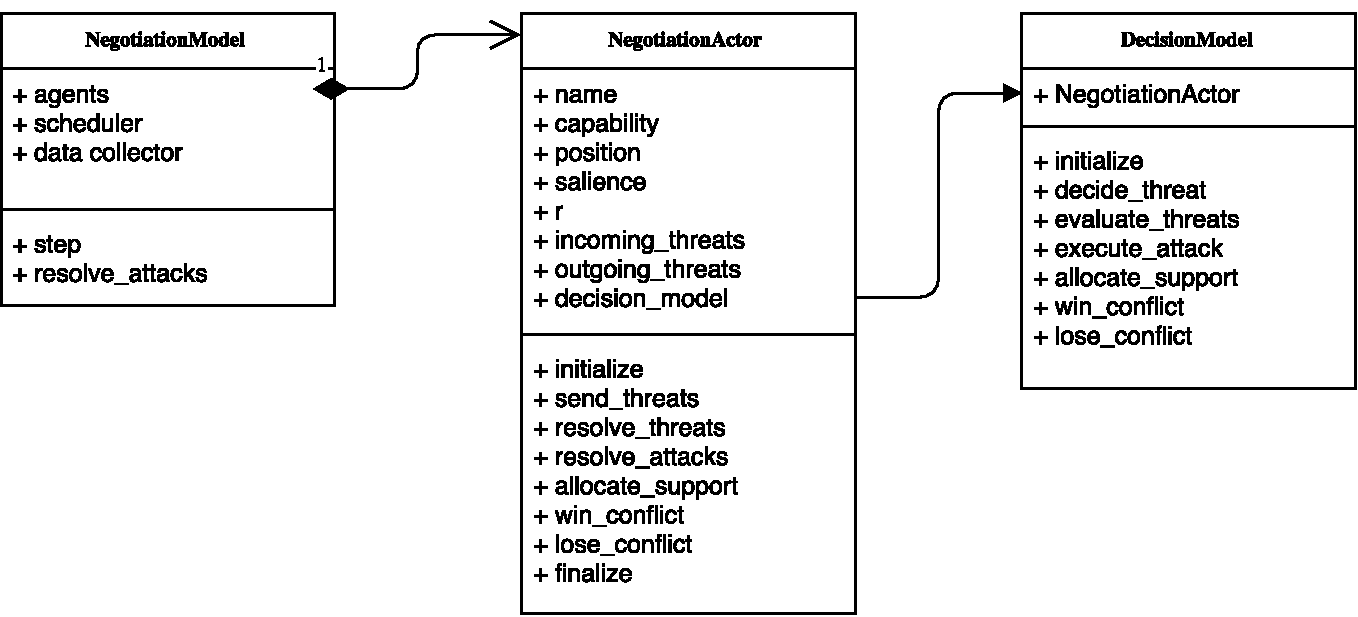
\includegraphics[width=\textwidth]{BDM_Reproduction/Figures/BDM_Architecture}
  \caption{Model Architecture}
  \label{fig:bdm_architecture}
  \figSpace
\end{figure}

\subsection{Details} \label{details}
%% Quick overview here?
\subsubsection{Initialization and Inputs} \label{initialization}

Each model instantiation is meant to simulate a particular issue under contention. Thus, we begin by identifying the issue of interest, and the actors we need to represent. In some cases, identifying the actors is simple: for example, all the states who are party to a particular formal negotiation process, or (in a retrospective simulation) all the states who participated in a particular conflict. In other cases, qualitative expertise (the modeler's own, or elicited from subject-matter experts) may be needed to determine who the relevant actors are.

For every actor, we must assign position, salience, and capability values. Like the list of actors, the actor properties may be derived from different sources. We may elicit subject-matter experts for their estimates, or utilize various quantitative datasets more objective or replicable measures. Capabilities are perhaps the easiest to measure objectively; the National Material Capabilities (NMC) dataset \citep{singer_1972,singer_1988} provides several calibrated measures of national power, aggregated into the Composite Index of National Capability (CINC). Position is harder to measure. One method is computing the similarity of states' alliance portfolios \citep{bdm_1975,bdm_1992,signorino_1999b}: the more similar the alliances that two states hold are, the closer their interests are presumed to align. There has not been, to the best of my knowledge, an attempt to formally estimate salience from data. It can either be set based on expert estimates, or treated as an unobserved random variable.

%% Submodels

\subsubsection{Risk Propensity Update ($\mathbf{R_0}$)} \label{risk_update}

Conceptually, actors wish to balance between their preferred issue outcome and their desire to be a part of a winning coalition. At one extreme, an actor may adhere to its own position regardless of the positions of the rest of the actors, and no matter how much power is arrayed against it. At the other extreme, an actor may completely abandon its preferred position and seek to position itself as close as possible to the current consensus or winning position. In practice, most actors are likely to fall somewhere between these two poles.

In order to estimate each actor's risk propensity, the model compares the actor's current security to the security of all other actors in the model. More formally:

\begin{equation}
    R_i = \frac{ 2 \sum\limits_j E^i(U_{ji}) - \max\limits_j \sum\limits_{k} E^i(U_{kj})  -  \min\limits_j \sum\limits_{k} E^i(U_{kj})}{\max\limits_j \sum\limits_{k} E^i(U_{kj})  -  \min\limits_j \sum\limits_{k} E^i(U_{kj})} \label{eq:R_0}
\end{equation}

In this equation, $E^i(U_{ji})$ refers to agent $i$'s perception of $j$'s expected utility of threatening $i$; the full expected utility calculation is specified in Equation \ref{eq:EU}. This result is then normalized as follows:

\begin{equation}
    r_i = \frac{1 - R_i/3}{1 + R_i/3}
\end{equation}

In the model as described in \citet{bdm_2002} and \citet{scholz_2011}, the risk propensity is recalculated at every step, with an initial assumption of $r_i=1$ for all actors. This means that risk propensity is not a fixed property of the actor, but emerges from the overall model state. This can be thought of as the risk propensity required to maintain the actor's current position.

\subsubsection{Expected Utility Calculation ($\mathbf{O_0}$)} \label{eu_calc}

The expected utility (EU) calculation is important enough to have given the model the name it is most often known as -- the Expected Utility Model. In each step of the model, the first decision facing each agent is whether to send an offer to each other agent, which they will do only if their expected utility is positive.

In order to compute the expected utility of threatening a particular target $j$, actor $i$ computes the utilities of the following potential outcomes:

\begin{enumerate}
    \item The actor threatens the target, and:

        \begin{enumerate}
        \item Enters into conflict and wins: 
            \begin{equation}
            U_s = 2 - 4(0.5 - 0.5|x_i - x_j|)^{r_i} \label{eq:u_s}
            \end{equation}
        \item Enters into conflict and loses:
            \begin{equation}
            U_f = 2 - 4(0.5 + 0.5|x_i - x_j|)^{r_i}
            \end{equation}
        \item The target capitulates without a conflict ($U_s$ again, as computed in Equation \ref{eq:u_s})
        \end{enumerate}
    \item The actor does not threaten the target, and:
        \begin{enumerate}
        \item The status quo continues:
            \begin{equation}
            U_{sq} = 2 - 4(0.5)^{r_i}
            \end{equation}
        \item The target moves towards the current median position $\mu$:
        \begin{equation}
            U_b = 2 - 4(0.5 - 0.25(|x_i-\mu|+|x_j-\mu|))^{r_i}
            \end{equation}
        \item The target moves away from the current median position $\mu$:
        \begin{equation}
            U_w = 2 - 4(0.5 + 0.25(|x_i-\mu|+|x_j-\mu|))^{r_i} \label{eq:u_w}
            \end{equation}
        \end{enumerate}
\end{enumerate}

Next, the actor assigns probabilities to each outcome. The probability of winning and losing the conflict are this actor's perception of the fraction of support allocated to its position as compared to the target's. For a conflict between agents $j$ and $k$, actor $i$'s support (or `votes') is computed as follows:

\begin{equation}
    v^{i}_{jk} = c_is_i (|x_i-x_k| - |x_i-x_j|) \label{eq:votes}
\end{equation}

When $v^{i}_{jk}$ is positive, $i$ supports $j$; negative, and $i$ supports $k$. In light of this, $i$'s perceived probability of a victory by $j$ in a conflict between $j$ and $k$ is:

\begin{equation}
P^i_{jk} = \frac{\sum\limits_{h|v^h_{jk}>0}v^h_{jk}}{\sum\limits_{h}|v^h_{jk}|} \label{eq:p_win}
\end{equation}

This probability calculation is also used to determine the median position. The model extends the \citet{black_1948} median voter calculation to account for the fact that each actor has a different `voting' power, and may cast a different number of votes (allocate a different level of support) in different bilateral contests. The median position $x^*$ is thus:

\begin{equation}
    x_i^* \equiv P^i_{*k} > 0.5 \text{ } \forall \text{ } k \in N
\end{equation}

Or, plainly, the position which is likely to defeat all other positions in bilateral contests.

The target's salience is used as the probability that it will yield to the threat, rather than enter into a conflict. Finally, the actor's perception of the probability of the target not moving at all is denoted $Q_i$; and of the target moving towards the median position if it does move is $T_i$. These appear to generally be held fixed for all agents in a given model instantiation, and as such become model parameters. 

Putting all the terms together gives us the full expected utility calculation. For convenience, the equation below omits all the full perception designation terms. The utilities are $i$'s perception of $j$'s utility of winning, losing, etc. $P$ is $i$'s perception of $j$'s probability of winning the conflict. 

\begin{equation}
    \label{eq:EU}
    \begin{split}
    E^i(j,k) = E^i(U_{jk}) = s_k (P U_s + (1-P)U_f) + (1 - s_k)U_s \\
    - Q_i U_{sq} + (1-Q_i)(T_iU_b + (1-T_i)U_w)
    \end{split}
\end{equation}

This EU value comes into play in several ways: first, at each step, agents issue an offer when the expected utility is positive -- that is, the agents expect a better outcome from issuing a threat than not issuing it. Second, it determines how each target of a offer responds, as the next section describes.

\subsubsection{Responding to Offers ($\mathbf{M_0, A_0}$)} \label{challenges}

Once all the actors have sent their offers, they decide on at most one offer to accept. The offer selection mechanism is perhaps the least specified of all the model components in any of the prior literature. I utilize the description provided by \citet{scholz_2011}, who argue that agents choose offers based on two criteria: the expected utility associated with each offer, and the distance it requires the target actor to move.

In this approach, agents initially evaluate the distance between their current position, and the position associated with the offer. Agents will choose offers where this distance is the smallest, preferring to accept offers requiring them to change position the least.

If there is a single closest offer, it is selected. However, if there are multiple offers with the same distance associated with them, the agent selects the most enforceable one -- that is, the one with the highest perceived expected utility on the part of the sender.

How agents actually change their position based on their accepted offer is determined by the combination of the source and the target's perceived expected utility of threatening one another. The recipient of a threat evaluates how much it believes it stands to lose or gain from a conflict, and how much it believes the sender of the threat stands to lose or gain, and decides accordingly. The combinations of perceived utilities may fall into one of several octants, as shown in Figure \ref{fig:octants}.

\begin{figure}
  \centering
  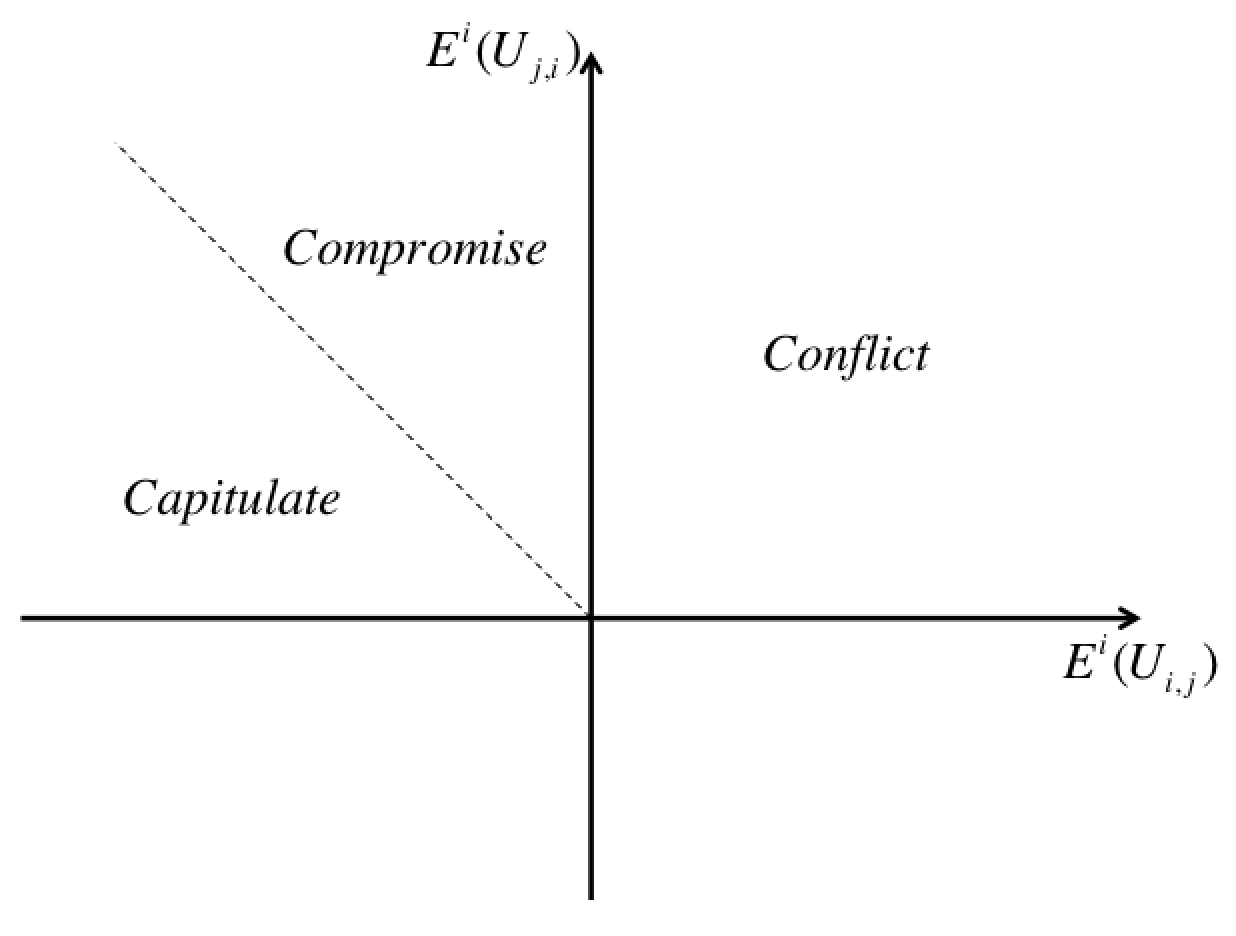
\includegraphics[scale=0.5]{BDM_Reproduction/Figures/Octants}
  \caption{Incoming Offer Categories}
  \label{fig:octants}
  \figSpace
\end{figure}

\begin{description}
    \item[Capitulate:] This octant is the region of the EUxEU space where the target's EU is negative, and has an absolute value greater than the positive EU of the source. More colloquially, the target stands to lose more than the attacker stands to gain. This indicates a decisive advantage for the source in case of a conflict; in the face of some advantage, the target yields completely, adopting the source's position as its own. 

    \item[Compromise:] In this octant, the target's EU is negative, but smaller in magnitude than the source's. In this case, the sender cannot enforce complete surrender, but can nevertheless coerce the target into changing its position towards that of the sender. The size of the step is determined by the ratio between the magnitudes of both actors' expected utilities, or more formally:
    
    \begin{equation}
        x_i^\prime = x_i + (x_j - x_i)\left\lvert\frac{E^i(U_{ji})}{E^i(U_{ij})}\right\rvert
    \end{equation}

    Thus, as the source's EU increases, the target agrees to increasingly better compromises.

    \item[Conflict:] The conflict quadrant consists of the region of the space where both actors' expected utility from a conflict is positive; in other words, conflict can occur only when both actors expect to gain from it. When actors choose to enter into a conflict with one another, the Conflict sub-model is called, as described below.

\end{description}

\citet{bdm_2002} notes that ``Each player is free to renege on a proposed deal so long as it can enforce another agreement or so long as someone else can enforce an agreement on it.'' In practice, the latter part of the sentence refers to the fact that actors choose only one incoming offer to accept; I interpret the first half to mean that actors need not change position if another actor accepted their offer and is changing position towards them. This resolves a situation I observed while developing and experimenting with the model, where actor A capitulated to actor B, while actor B simultaneously capitulated to actor C -- in effect, B coerces A into holding a position A itself is simultaneously abandoning.

\subsubsection{Conflicts ($\mathbf{W_0}$)}

Conflicts occur when both actors see positive expected utility from a conflict with the other, leading them to choose each other's offer, and when neither agent reneges due to another agent accepting their offer. For each conflict occurring in a given step, all agents contribute some fraction of their capabilities to one side or the other, as described in Equation \ref{eq:votes}, yielding the probability given in Equation \ref{eq:p_win}. The model stochastically chooses the winner with that probability, and the loser updates their position to that of the winner. The assumptions regarding conflicts are discussed in much more detail in Section \ref{bdm_discussion}.

\section{Model Validation and Verification} \label{model_vv}

The description above appears, to the best of my ability to ascertain, to be a faithful representation of the BDM Expected Utility model, as presented in the prior literature. However, as documented by \citet{scholz_2011}, not only has the model never been fully specified, but several components of it have been modified over time. In this section, I attempt to validate my implementation against two sets of inputs and outputs from the prior literature -- and I should note up-front that in neither of these cases do I successfully fully reproduce the original reported results. In light of this, I conduct a deep dive into one of the model runs and provide a detailed walk-through of a single model step. This serves to verify that the model is working as expected, as well as to build the reader's intuition and understanding of the model's behavior and dynamics.

\subsection{Reproduction of Prior Results} \label{verification}

A natural way to validate that the model described here successfully replicates the original is by reproducing prior results from known inputs. There are several models where the inputs are fully specified (or very nearly so) to allow for such replication attempts. For example, \citet{scholz_2011} use the data from \citet{bdm_1994}, an application of the model to European vehicle standard negotiations, and demonstrate the reproduction of several model outputs. I attempt to reproduce this replication, as well as the China democratization example examined in \citet[chapter 6]{bdm_2002}. Since the latter model in particular involves a stochastic element, we cannot reproduce the exact same results without knowing outcomes of the various random draws; instead, I examine the distribution of results across multiple model runs. 

The case examined by \citet{scholz_2011} involves ten members of the European Community (the precursor to the European Union), negotiating over when to apply new emission regulations to mid-size automobiles (the full inputs are provided in Table \ref{table:eg_agent_data}). This case provides a good starting point, since there is minimal stochasticity in the model implementation -- the inputs, including the saliences, are all fixed. The \citet{scholz_2011} replication was validated in two ways: by comparing the median position, and the quadrants pairs of agents fall in, to those produced by the original model. The \citet{scholz_2011} model perfectly reproduced the median position changes reported in \citet{bdm_1994}. Figure \ref{fig:model_comparison}, compares those median positions to those generated by my own implementation. The comparison highlights the fact that the original model produces cyclic behavior which mine does not: certainly a richer dynamic, but not one with any external reason for us to believe it to be correct. (The observed historic outcome, 8.833 years, corresponds to approximately 0.8 on the normalized issue space, which neither model converges to).

\begin{figure}
  \centering
  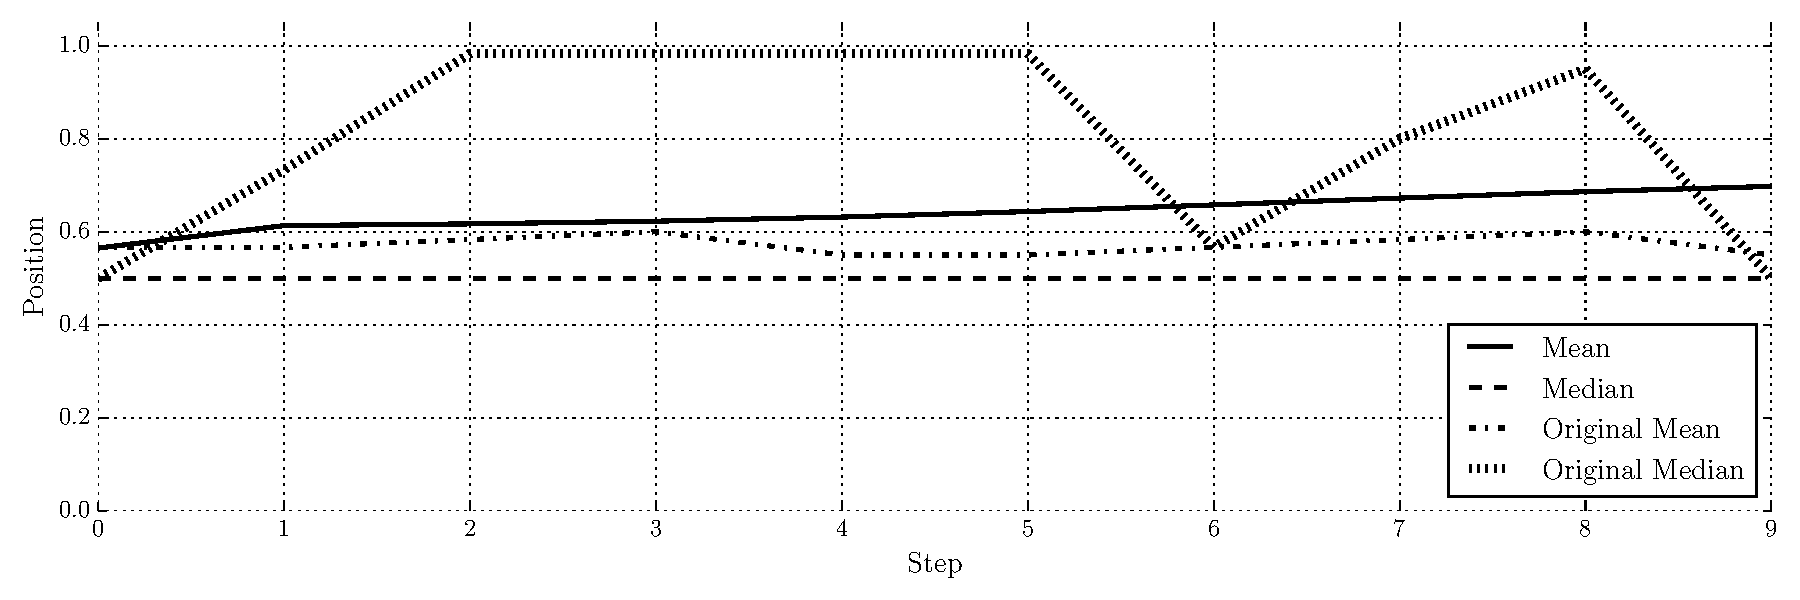
\includegraphics[scale=0.5]{BDM_Reproduction/Figures/ModelComparison}
  \caption{Original and Replication Model Comparison}
  \label{fig:model_comparison}

  \figSpace
\end{figure}

Stronger evidence still that the \citet{scholz_2011} model replicates the BDM results comes from the octant comparison, comparing the expected utilities of between pairs of agents at the first step of the model. As the paper notes, there is a vanishingly-small probability of the same octant configuration resulting by chance. My own model does not replicate these octant configurations. One example is shown in Figure \ref{fig:octant_comparison}, with Belgium as the focal actor -- the position of each other agent is Belgium's expected utility from challenging it, and its own expected utility from challenging Belgium.

\begin{figure}
    \centering
    \begin{subfigure}{0.32\textwidth}
        %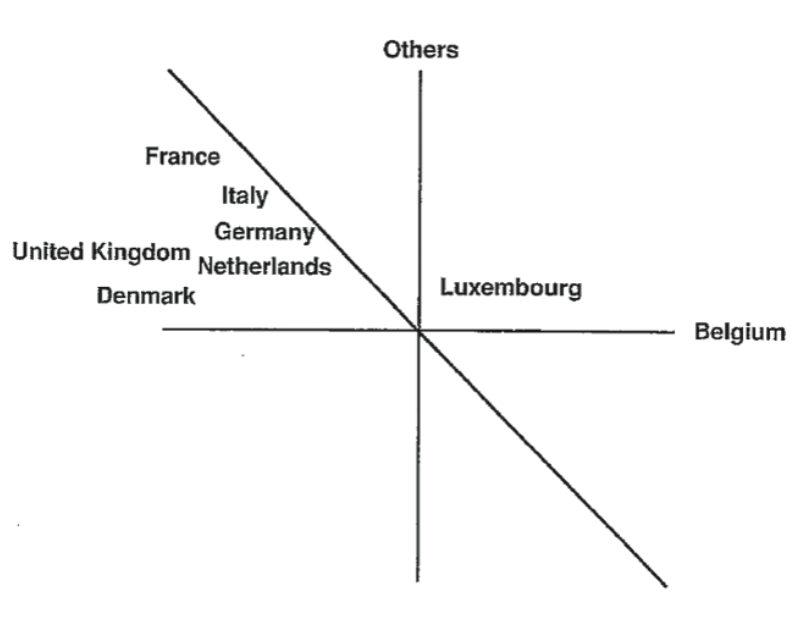
\includegraphics[width=\textwidth]{BDM_Reproduction/Figures/Octants_BDM94}
        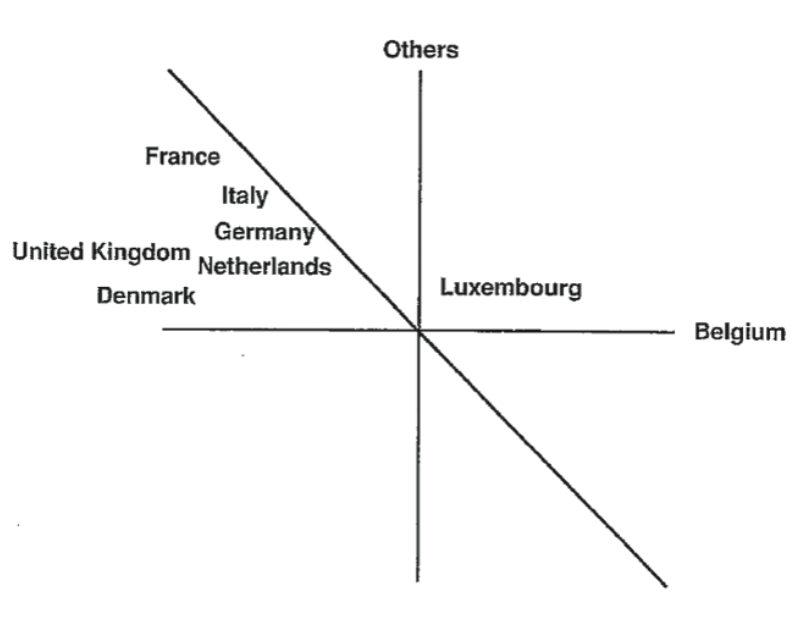
\includegraphics[height=5cm]{BDM_Reproduction/Figures/Octants_BDM94}
        \caption{\citet{bdm_1994} Expected Utilities}
    \end{subfigure}
    \begin{subfigure}{0.32\textwidth}
        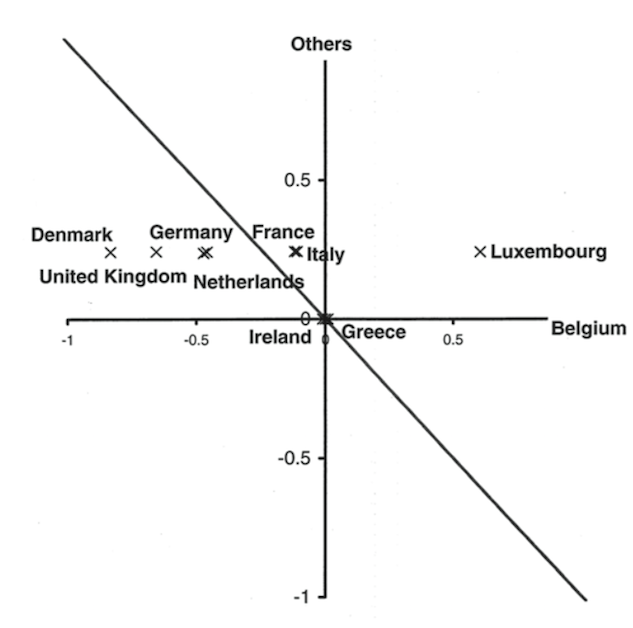
\includegraphics[height=5cm]{BDM_Reproduction/Figures/Octants_Scholz11}
        \caption{\citet{scholz_2011} Expected Utilities}
    \end{subfigure}
    \begin{subfigure}{0.32\textwidth}
        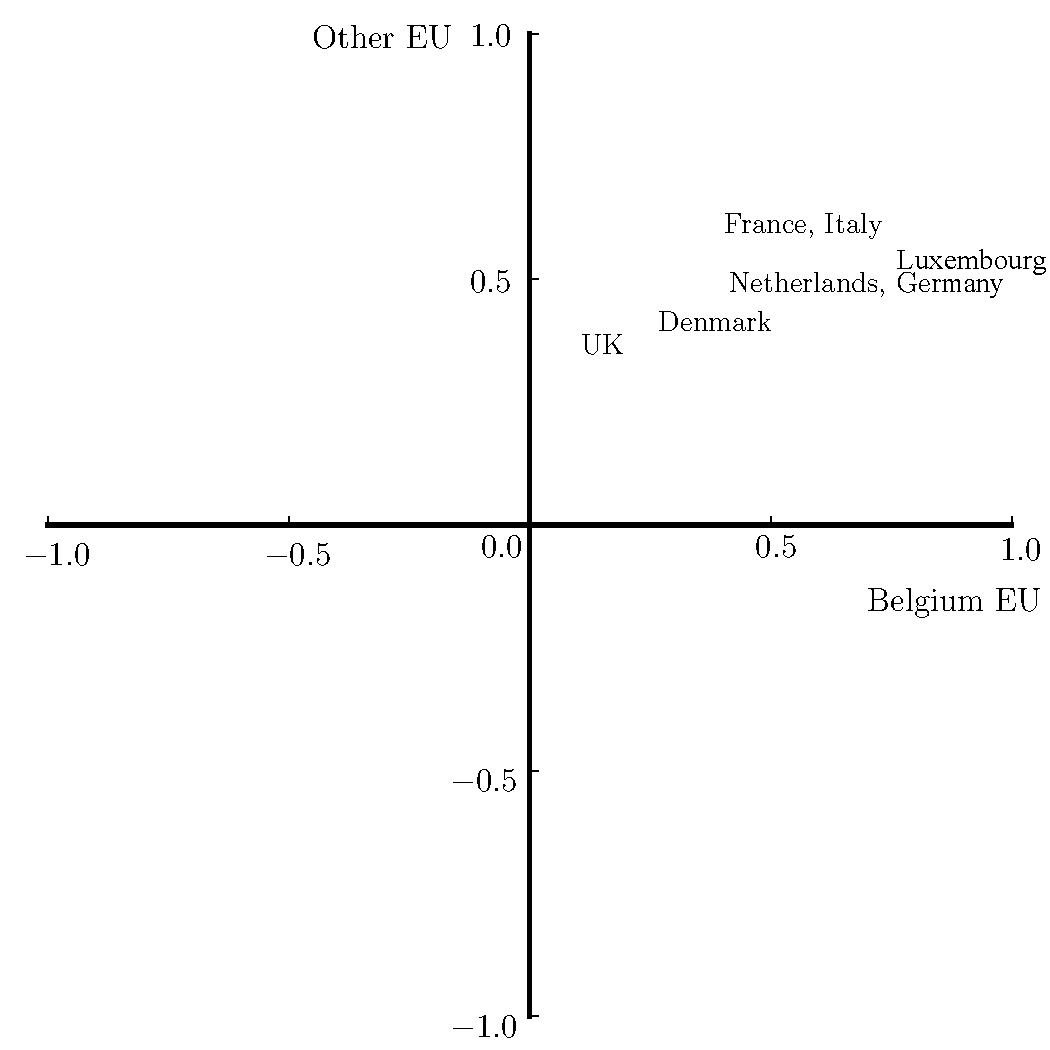
\includegraphics[height=5cm]{BDM_Reproduction/Figures/OctantComparison}
        \caption{Model reimplementation}
    \end{subfigure}

    \caption[Octant Comparison]{Octant Comparison, with Belgium as Focal Agent}
    \label{fig:octant_comparison}
    \figSpace

\end{figure}

A close comparison of the models suggests that the Scholz octant configuration is driven by far smaller probabilities of victory that the model produces, normalized by all possible votes rather than just the ones on the conflict at hand. This probability form appears to contradict the form of probability calculations provided in \citet{bdm_1997,bdm_2002}, and (more importantly) a basic rule of probability: if there are two possible outcomes (in this case, actor $i$ wins or actor $j$ wins), their probabilities must sum to 1. There are, then, two alternatives: one is that the Scholz model is successfully replicating an erroneous BDM model implementation; the other is that there is some other mismatch between the models which is producing matching octants. There are two, somewhat contradictory, preliminary conclusions we can take from here: that the overall model is sensitive to changes in specific sub-models, and that it is nevertheless robust enough to produce similar results even when these sub-models differ, and produce substantively different interactions.

Furthermore, while the Scholz model successfully replicates specific features of this one particular model instantiation, this success does not translate to other cases. \citet{scholz_2011} note that their implementation fails to replicate another case, presented in \citet{bdm_1997}. Experiments on my part confirm that it also fails to replicate the following cases, which I will describe next.

The next case I use is the Chinese democratization example, presented in chapters 3 and 6 of \citet{bdm_2002}. In this case, the model is being instantiated is attempting to predict the dynamics of internal political reform in the People's Republic of China. The agents here are a mix of individuals, organizations, loose factions (e.g. ``Students and Intellectuals''), and foreign countries. \citet{bdm_2002} reports model median positions by step for several model instantiation. However, as part of this particular case, agents' saliences are randomized each step, with 20\% probability each; the reported results do not specify which saliences were changed and how. This makes it effectively impossible to attempt to replicate the exact same model run. To overcome this, I generate many more model runs: 50 of the Scholz model, and 100 of my own. I start each run with the initial conditions provided in \citet{bdm_2002}, and randomize agent salience values as described. This yields a distribution of models, and in particular a distribution of medians. Figure \ref{fig:china_medians} shows the distributions of these medians, as well as a dotted line indicating the reported median\footnote{This median value was taken from \citet[chapter 3]{bdm_2002}; chapter 6 provides only a chart of medians from several runs, but not precise values. However, the chart shows values close to the one used here.}. In this case, the models produce similar, though not identical, distributions to one another -- and neither comes close to the reported values. This indicates that the Scholz model is not a perfect replication of the original model as implemented. Furthermore, it suggests that we may need to be cautious about using any single set of reported model results as `ground truth.'

In light of these results, and of the reported changes in the variations of the original model, I believe that validating the model reimplementation directly against reported model outputs is not a tenable option. Nevertheless, I believe that the model I have implemented correctly captures the core sub-models of the original, and provides a sufficiently solid basis to proceed with this analysis.

\begin{figure}
    \centering
    \begin{subfigure}{0.49\textwidth}
        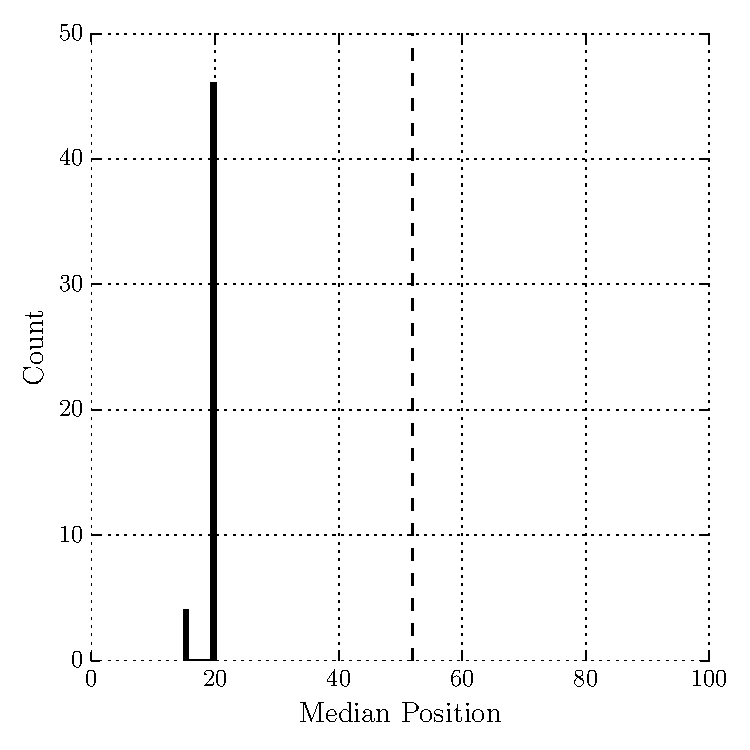
\includegraphics[width=\textwidth]{BDM_Reproduction/Figures/Scholz_ChinaModel}
        \caption{\citet{scholz_2011} Median Positions}
    \end{subfigure}
    \begin{subfigure}{0.49\textwidth}
        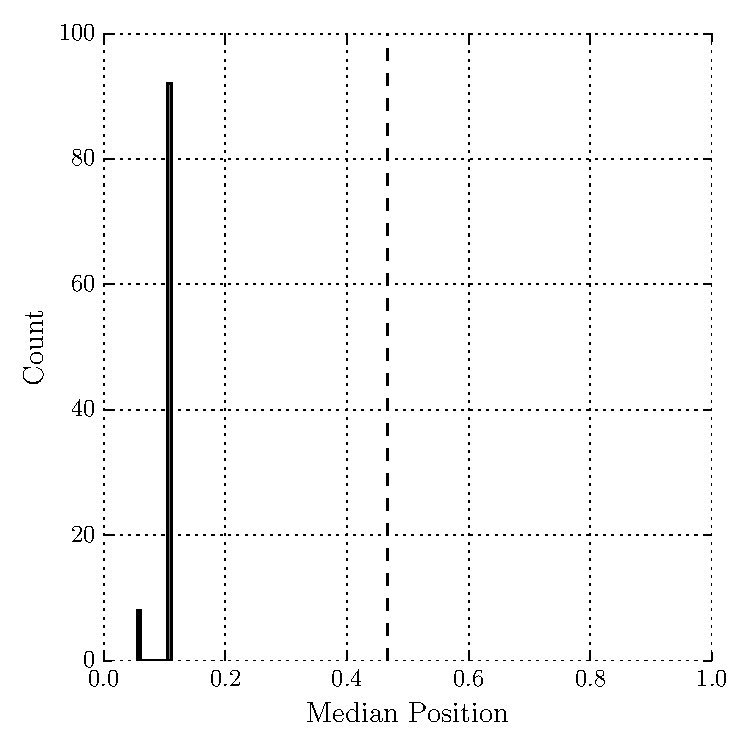
\includegraphics[width=\textwidth]{BDM_Reproduction/Figures/New_ChinaModel}
        \caption{Reimplemented Model Median Positions}
    \end{subfigure}

    \caption[Chinese Democratization Model Medians]{Chinese Democratization Model Medians, at the End of Step 2}
    \label{fig:china_medians}
    \figSpace
\end{figure}


\subsection{Deep Dive} \label{deep-dive}

In order to understand how the model behaves, it is valuable to take a close look at the sequence of actions in a single iteration. This will also serve as a method of verification, ensuring that the model is not producing unexpected or incorrect behaviors. In order to do so, I will continue to use the case presented above, of the negotiation over European Community vehicle standards. I choose this example in particular since it has already been well-studied: first by \citet{bdm_1994} directly, then by \citet{scholz_2011} as the key case for testing their replication of the original BDM model; and finally by \citet{mckibben_sanders_2014} testing the replication of the replication. Furthermore, the number of agents is small enough to make the interactions amenable to direct human examination, and the position space has a straightforward, numeric interpretation: the years before the regulations are applied. The agent initial positions, capability and saliences were all determined by consultation with subject-matter experts.

\begin{table}
\centering
\caption{Example Model -- Agent Data}
\label{table:eg_agent_data}
\begin{tabular}{lccc|c}
    \hline
    Name &  Capability &  Position &  Salience & $r_{i,0}$ \\
    \hline
    Netherlands &        0.08 &       0.0 &       0.8 & 1.12 \\
        Belgium &        0.08 &       0.5 &       0.4 & 1.00 \\
     Luxembourg &        0.03 &       0.0 &       0.2 & 0.50 \\
        Germany &        0.16 &       0.0 &       0.8 & 1.12 \\
         France &        0.16 &       1.0 &       0.6 & 1.02 \\
          Italy &        0.16 &       1.0 &       0.6 & 1.02 \\
             UK &        0.16 &       1.0 &       0.9 & 2.00 \\
        Ireland &        0.05 &       0.5 &       0.1 & 0.65 \\
        Denmark &        0.05 &       0.0 &       1.0 & 1.45 \\
         Greece &        0.08 &       0.5 &       0.7 & 1.56 \\
    \hline
\end{tabular}
\tableSpace
\end{table}

Initially, the model computes the risk propensity coefficients shown in Table \ref{table:eg_agent_data}. Note that indeed one agent, the UK, has a value of $r=2.0$ and another one, Luxembourg, has $r=0.5$; as agents are computing their risk propensity in comparison with one another, at least one agent will always have each of these values, in any step of any given model instantiation.

Next, the agents estimate their expected utility of threatening all other agents, sending offers where those expected utilities are greater than zero. These EUs are given in Table \ref{table:eg_eu}. The important thing to note here is that the majority of directed dyads have a positive EU value -- which means that all those dyads will have threats issued across them. 

\begin{table}
\centering
    \caption[Example Model -- Expected Utilities]{Example Model -- Expected Utilities, step$=0$}
    \label{table:eg_eu}
    \begin{tabular}{r|cccccccccc}

        Source  \textbackslash Target &  Bel. &  Den. &  Fra. &  Ger. &  Gre. &  Ire. &  Ita. &  Lux. &  Net. &    UK \\
        \hline
        Belgium     &      -- &     0.27 &    0.40 &     0.41 &    0.00 &     0.00 &   0.40 &        0.85 &         0.41 &  0.11 \\
        Denmark     &     0.39 &      -- &    0.08 &     0.00 &   -0.00 &     0.79 &   0.08 &        0.00 &         0.00 & -0.61 \\
        France      &     0.60 &     0.28 &     -- &     0.62 &    0.29 &     0.90 &   0.00 &        1.64 &         0.62 &  0.00 \\
        Germany     &     0.47 &     0.00 &    0.46 &      -- &    0.08 &     0.86 &   0.46 &        0.00 &         0.00 & -0.23 \\
        Greece      &     0.00 &     0.13 &    0.27 &     0.28 &     -- &     0.00 &   0.27 &        0.74 &         0.28 & -0.04 \\
        Ireland     &     0.00 &     0.30 &    0.42 &     0.43 &    0.00 &      -- &   0.42 &        0.80 &         0.43 &  0.17 \\
        Italy       &     0.60 &     0.28 &    0.00 &     0.62 &    0.29 &     0.90 &    -- &        1.64 &         0.62 &  0.00 \\
        Luxembourg  &     0.46 &     0.00 &    1.45 &     0.00 &    0.18 &     0.74 &   1.45 &         -- &         0.00 &  0.76 \\
        Netherlands &     0.47 &     0.00 &    0.46 &     0.00 &    0.08 &     0.86 &   0.46 &        0.00 &          -- & -0.23 \\
        UK          &     0.35 &    -0.70 &    0.00 &    -0.36 &    0.04 &     0.65 &   0.00 &        0.66 &        -0.36 &   -- \\
    \end{tabular}
    \tableSpace
\end{table}

\begin{table}
\centering
    \caption{Accepted Offers}
    \label{eg_offers}
\begin{tabular}{lll}
    \hline
    Agent &  Accepted Offer & Category \\
    \hline
    Netherlands & Belgium & conflict \\
    Belgium & Netherlands & conflict \\
    Luxembourg & Belgium & conflict \\
    Germany & Belgium & conflict \\
    France & Belgium & conflict \\
    Italy & Belgium & conflict \\
    Ireland & Netherlands & conflict \\
    Denmark & Greece & compromise \\
    Greece & UK & compromise \\
    \hline
\end{tabular}
\tableSpace

\end{table}

Table \ref{eg_offers} shows which offer each agent accepts, and what category each one falls into. Immediately, we notice that five agents all choose to enter into conflict with Belgium. Note that Belgium's position is exactly in the middle of the issue space, and it has lower salience than Greece, the other agent holding the same position, making it an appealing target. For a conflict to occur, Belgium must choose one of them -- and indeed chooses the Netherlands, which leads to a conflict. Meanwhile, Denmark chooses to compromise with Greece and update its position towards it, while Greece chooses to compromise with the UK. However, recall that agents renege on offers if another agent has accepted their own offer in a more preferable way. In this case, since Denmark has chosen to compromise with Greece, Greece in turn backs out from its decision to compromise with the UK, and will not update its position after all.

The conflict between Belgium and the Netherlands happens before Denmark updates its position. Each agent contributes capability to one side or the other, as governed by Equation \ref{eq:votes}; these contributions are shown in Table \ref{table:contributions}. Note that even the two actual actors entering into the conflict do not allocate their full capabilities: they are scaled once by their salience, and again by the distance between their positions. Putting the total values into Equation \ref{eq:p_win} yields a probability of victory of 0.63 for Belgium, and thus 0.37 for the Netherlands. The model uses these probabilities to randomly select the winner; if Belgium wins, the Netherlands updates its position to 0.5, and if the Netherlands wins Belgium updates its own position to 0. At this point, Denmark will update its own position to compromise with Greece. Then, the next round begins.

\begin{table}[h!]
\centering
    \caption{Capability Contribution -- Belgium vs Netherlands}
    \label{table:contributions}
\begin{tabular}{lcc}
    \hline
    Agent &  Belgium & Netherlands \\
    \hline
    Netherlands & 0 & 0.032 \\
    Belgium & 0.016 & 0 \\
    Luxembourg & 0 & 0.003 \\
    Germany & 0 & 0.064 \\
    France & 0.048 & 0 \\
    Italy & 0.048 & 0 \\
    UK & 0.072 & 0 \\
    Ireland & 0.0025 & 0 \\
    Denmark & 0 & 0.025 \\
    Greece & 0.028 & 0 \\
    \textbf{Total} & \textbf{0.2145} & \textbf{0.124} \\
    \hline
\end{tabular}
\tableSpace

\end{table}

%Table \ref{eg_offers} shows which offer each agent accepts, and what category each one falls into. Immediately, we notice that six agents all choose to enter into conflict with Belgium. Note that Belgium's position is exactly in the middle of the issue space, and it has lower salience than Greece, the other agent holding the same position, making it an appealing target. For a conflict to occur, Belgium must choose one of them -- and indeed chooses the Netherlands, which should lead to a conflict. However, recall that agents renege on offers if another agent has accepted their own offer in a more preferable way. In this case, Denmark agrees to compromise with Belgium, meaning that Belgium will in turn back out of its conflict with the Netherlands. In the end, in fact, no conflicts occur, and the only movement is by agents moving unilaterally: Greece, capitulating, and Denmark, compromising.

\section{Model Discussion} \label{bdm_discussion}

Examining the description of the model above, we can see clearly that it is in fact an agent-based model: the actors are the agents, interacting with each other in discrete steps according to a set structure. Each agent is endowed with several properties, some public and some private, making it natural to model them using object-oriented design. Indeed, the focus on the utility calculations in much of the prior literature elides the deeply computational nature of this model. It is anchored not only in game-theoretic logic, but on embedded assumptions which have a substantial effect on the model's behavior, and which, when articulated in code, are easy to experiment with. 

The model, like many agent-based models, can be separated into two layers: the agents' external behavior with regard to one another, and their internal decisionmaking process. 

Externally, agents send threats to some other agent. A threat has no information specifically attached (though of course the target has access to the public information on the source of the threat) -- it is simply boolean; either a source has issued a threat to a target, or it has not. Next, all agents choose how to change their public positions in response to the incoming threats -- and these choices are public, and simultaneously become common knowledge. When two agents have chosen conflict with one another, conflicts occur and are resolved. Finally, agents update their stated positions based on the offers and conflict outcomes, before the sequence starts over. These steps happen in sequence with one another, but that all agents act simultaneously within each step.

Note that at no point in this sequence do utilities, expected or otherwise, come into play. The utilities are computed, and applied, internally by agents to drive their decisionmaking, choosing who to send threats to and how to respond to them. We can easily imagine other beliefs and heuristics guiding agent decisions besides the ones that have been chosen here. Even the sequence of events itself is not necessarily fixed.

In this section, I will discuss several of the model assumptions in greater depth. I also propose sub-model variants which implement alternative assumptions. The object-oriented nature of the model means that a single sub-model to be replaced without modifying any other aspect of it. This, in turn, allows us to instantiate different model variants with the same initial conditions and directly compare their dynamics and outputs -- and, in turn, use these to understand how the assumptions drive the model as a whole.

\subsection{Expected Utility}

While the expected utility calculation (Equation \ref{eq:EU}) is important enough to give the model its name, I note that this calculation is largely heuristic in nature. The probability of winning or losing $P$ (as computed in Equation \ref{eq:p_win}) is based on the best possible approximation. The inclusion of the salience term as a probability, however, is much more obviously a heuristic. The source of a potential threat uses salience as the probability of the target yielding to that threat. However, salience does not play a similar role in the threat response side of the model; in fact, it is possible for an agent to have low salience and high probability of winning a conflict, and hence high EU, due to support from other agents. Simply put: agents are modeled as making an estimation that is plausible on its face, but that nevertheless does not reflect the reality of the model itself. 

$Q$ and $T$ are more clearly broad heuristics: they are not as specifically tied to the behavior of a particular agent, but are approximate, coarse-grained estimates of the behavior of the world overall. While \citet{bdm_2002} suggests that agents update their belief about the world in response to the outcome of each round, no such learning rule is provided. $Q$ and $T$ provide candidates for such updating: for example, the agents could use the fraction of agents that moved last round as $Q$, or update their belief in a Bayesian fashion based on a prior probability distribution for $Q$. Alternatively, we may note that any given model potentially represents one issue among many which the actors are addressing at once or in rapid sequence, and suggest that $Q$ and $T$ represent heuristics developed across all issues.

\subsection{Conflict and Coercion} \label{conflict_coercion}

The Conflict outcome deserves special attention here. Conflict, and especially war, plays an outsize role in the study of international relations, and indeed in world history. Being able to predict the outbreak of conflicts would be a particularly powerful result from this model; in fact, the risk propensity and probability of victory sub-models were originally developed precisely for such predictions \citep{bdm_1985}. For these reasons, it is important to understand precisely when the model predicts conflicts will occur, and how to interpret such predictions.

There are several ways of handling a conflict and its outcome. The method put forward in \citet{scholz_2011} involves comparing both agents' expected utility from the conflict; the winner is the one with the greater EU, and the loser changes position to match the winner's. I believe this approach is incorrect, for several reasons. EU incorporates a specific term for probability of winning, but also the terms for movement absent a threat -- which, if a conflict is actively breaking out, are no longer relevant. Furthermore, if a conflict is already occurring, it is unclear why the salience should continue to have a probability-like effect. The calculation for $P$ (Equation \ref{eq:p_win}) clearly implies that the probability of winning and losing is tied primarily to the total capability brought to bear, not the expected utilities associated with them.
%% Smooth the transision
However, these are secondary objections. Changing position is, ultimately, a decision that is internal to an actor. Allowing one agent to directly change another agent's position would breach the division between agents' external actions and internal decisionmaking. This is not how coercion has generally been understood. Coercion, as described by \citet{schelling_1966}, involves one actor presenting another, explicitly or implicitly, with a choice of complying with some demand or facing some punishment. Schelling describes this punishment primarily as  `pain' or `hurt' -- in other words, disutility. Importantly, in this view, the punishment need not degrade the target's capabilities, or eliminate it as a threat; it must simply impose a cost that is greater than the cost of complying with the given demand. If we examine militarized conflicts in particular, only a minority end with one side completely changing its orientation -- for example, the Second World War led to Japan's conversion by force from being an enemy of the United States to its ally \citep{schaller_1997}, and Tanzania's invasion of Uganda in 1978-79 successfully replaced the regime of Idi Amin with one friendly to Tanzania's interests \citep{acheson_2001}. However, in the majority of cases, even those involving what Schelling describes as `brute force' where one side wrested material gains from the other (such as in the Falklands or Gulf Wars), the other side's overall geopolitical orientation remained largely unchanged; certainly, they did not become allies of the power which defeated them.

The expected utility calculation, and its role in the model, is compatible with this view. There is an explicit negative utility to losing a conflict, which the agents attempt to avoid. The greater this threat -- the lower the overall expected utility of a conflict -- the more likely the agent is to capitulate entirely. Conflict cannot reduce agents' capabilities, or remove them from the model, suggesting that the disutility of losing bears more resemblance to Schelling's concept of `punishment' than `brute force.' Though the utilities associated with winning and losing a conflict are directly tied to the difference between the agent positions positions, this does not necessarily imply that the agents must change position upon losing. If the cost of losing a conflict is solely having one's position changed, what motive do actors in the `Capitulate' octant have to indeed capitulate, rather than embrace a chance, however slight, of changing the source's position through conflict? If a conflict does not change agent positions, it follows that these utilities are exogenous to the utility directly gained by an agent to have support at its current position. And indeed, in general, political actors do gain utility from winning (or succeeding in) a conflict: in the form of increased internal public support, prestige, credibility, and potentially an improved power ratio compared to the loser, while failing at a conflict carries the inverse costs \citep{bratton_2005}. Furthermore, both the means and the stakes of conflict will not be the same for close allies and rivals. Agents may attempt to coerce an ally, but are unlikely to use harsh measures which will risk harming the ally substantially and thus undermining their own position; similarly, the gains from inflicting such lesser costs on an ally will be less than those of inflicting greater losses on an enemy. 

We must note, of course, that the interpretation of conflict varies based on the particular scenario and issue under consideration. In modeling a negotiation over regulatory issues, conflict is highly unlikely to be military. However, in modeling geopolitical contests, conflicts may range from diplomatic snubs to economic sanctions to all-out war. Even military conflicts range in severity. A border clash, or targeted airstrikes, may inflict some costs on the target, but are unlikely to have direct system-wide effects. However, armed conflict between nuclear superpowers, as is a potential outcome in the \citet{bdm_1998} Cold War model (discussed in detail in the following chapter), runs the risk of consequences far outside the scope of this model.

Finally, the model elides the difference between when agents decide to engage in conflict and when the conflict, in fact, occurs. An implication of the offer-choice mechanic is that conflict occurs only when both parties choose to engage in it. This seems to remove the possibility of unilateral attacks. Furthermore, both parties to a conflict estimate the capability contribution of all other actors based on the parties' own risk propensity, and the agents' current positions. It seems reasonable that, once a conflict is initiated, other agents actually contribute capability based on their own decision rule -- and in particular, based on their own risk propensity. Here the precise scheduling of the conflicts compared to the rest of the model come into play: if conflicts occur \emph{after} agents change their positions in response to threats, their contribution of resources, and even the side to which they will contribute, may differ from their contributions before moving.

Based on this discussion, I propose two new sub-model variants. As these variants appear better grounded in prior theory than the baseline, I hypothesize they will produce better correspondence with empirical data.

\textbf{Conflict without position changing ($\mathbf{W_1}$):} Under this conflict sub-model variant, agents' positions are not changed when they lose a conflict. 

\textbf{Positions update before conflicts ($\mathbf{T_1}$):} Under this schedule variant, conflicts occur only after agents have moved in response to offers. This means that by the time a conflict occurs, the balance of power has shifted from what it was when the original threat was made.

\textbf{One-way attacks ($\mathbf{A_1}$):} This attack decision model variant removes the requirement for both agents to choose the other's offer for a conflict to be initiated. In this variation, an agent can attack any other agent it had threatened previously in this model step. However, it adds an additional decision-point, before attacks actually occur. At this decision point, the agent evaluates a modified form of the expected utility, which removes the uncertainty factors as to the target's response to the threat.

\begin{equation}
    EU_i^\prime(i,j) = P U_s + (1-P)U_f - U_sq
\end{equation}

Depending on when the agents new positions take effect, $P$, $U_s$ and $U_f$ may all be different from the values calculated at the offer-sending phase. If either the source or the target have changed position, the utilities of victory and defeat will be different as well; furthermore, if other agents have changed position, the direction and magnitude of support they are expected to provide will also have changed, changing the value of $P$ as well.

\subsection{Risk Propensity}

The risk propensity model attempts to estimate the risk an agent is willing to endure in pursuit of a preferred outcome; however, this is not directly risk propensity in the traditional economic sense (i.e. a relationship between a probability and the potential payoff an agent would require to wager on it), but in the political sense: how exposed the agent is willing to be to the possibility of being attacked, or simply left out of a winning coalition, in order to advocate for its preferred position or outcome. \citet{bdm_2002}, citing \citet{lamborn_1991}, describes this as a tradeoff between political satisfaction and policy satisfaction. When an agent is very secure, it is assumed to have chosen that secure position due to a low risk propensity; when it is insecure, this is taken as a revealed higher risk propensity.

Risk propensity is a key place where agents mirror-image: assuming that the other agents will make decisions the same way as they themselves do \citep{heuer_2001}. When agents estimate other agents' expected utility from an offer (Equation \ref{eq:EU}) they do not have access to the other agent's risk propensity, and so use their own instead, as detailed in Equations \ref{eq:u_s}--\ref{eq:u_w}. Mirror-imaging is a well-documented phenomena in humans \citep{meltzoff_2003}, and is also one of the cognitive traps intelligence analysts are frequently warned against \citep{heuer_2001} -- this suggests that it is not an unreasonable assumption for capturing real behavior. Nevertheless, risk propensity in this model is not an inherent property of the agent but emerges from the current configuration of positions. Thus, it is not at all clear whether we ought to expect organizations (or the individuals who compose them) to mirror-image on a dynamic, second-order property.

The form of the risk propensity calculation itself is explicitly grounded in Prospect Theory \citep{kahneman_1984,mcdermott_2001} in that it compares the agent's current security to two framing values: the best and worst possible security values for the agent. This helps explain why this value is recalculated each step: the best and worst security values may well have changed. This is expressed in a more generalized from of Equation \ref{eq:R_0}, using a non-specific security metric:

\begin{equation}
    R_i = \frac{ 2 security_i - \max\limits_j (security_j)  -  \min\limits_j (security_j)}{\max\limits_j (security_j)  -  \min\limits_j (security_j)}
\end{equation}

The original model measures security level as the sum of incoming expected utilities against an agent, or more formally:


\begin{equation}
    security_i = \sum_{j \in N} EU_i(j, i)
\end{equation}

Using this measure, a higher number (worse security) indicates more, and more powerful, potential attacks at the agent's current position.

I propose an alternative security level metric: the summed probabilities of successful attacks. This has the advantage of not relying on other's potential gain and loss; furthermore, unlike EU, probabilities are strictly positive, and thus negative values cannot reduce this value.  This metric was also adopted by \citet{wise_2015a}, as well as by another similar model variant reported to me by private communication. Formally, this security metric is:

\begin{equation}
    security_i = \sum\limits_{j \in N} P_i(j, i) \label{eq:r1_security}
\end{equation}

Next, consider the range of alternatives. In the original, this range is the security levels of all the other agents, or:

\begin{equation}
    (\min\limits_{j \in N} (security_j), \max\limits_{j \in N} (security_j))
\end{equation}

This method assumes that agents' risk propensities are relative to those of other agents. In particular, it has the consequence that one agent will always have the maximum possible risk propensity, while another will always have the minimum value. The alternative I introduce compares each agent's positions not to those of other agents, but to other possible positions the agent itself could hold, while holding all other agent positions constant. This follows the methodology used in \citet{bdm_1985}, as well as \citet{bdm_1992} and \citet{bennett_2000b}, and appears true to the description in \citet{bdm_2002} of examining ``the most political welfare... and the least the actor could have realized.'' Thus, the minimum and maximum security positions are defined as:

\begin{equation}
   (\min\limits_{x \in {[0, 1]}} (security_{i|x_i=x}), \max\limits_{x \in {[0, 1]}} (security_{i|x_i=x})) \label{eq:r1_range}
\end{equation}

This follows from an assumption that if an agent is holding a position which reduces their security they are more risk-accepting, while a position which increases their security indicates less risk propensity. Note, however, that it still cannot distinguish between an actor whose security-maximizing position is due to risk aversion from one which simply has a preference for that position separate from its degree of risk propensity. 

Putting these two variants together, I designate the risk-acceptance updating sub-model which utilizes Equations \ref{eq:r1_security} and \ref{eq:r1_range} as $\mathbf{R_1}$.

\subsection{Offer Selection}

Much like the expected utility calculation itself, the mechanism for offer selection and position updating is also a heuristic. It assumes that agents associate a particular potential position with each incoming offer, and will only select their new position from among those options. Furthermore, the model assumes that agents whose offers are not selected, or whose offers are reneged on, will simply accept this -- even when they have the coercive capability to force the target to change position. Yet this reneging rule has the effect of substantially reducing the frequency of agents actually changing their position.

I experiment with two alternative heuristics which address these issues. The first is simply stated: agents choose offers according to the original rules, but do not renege even if another agent has accepted their own offer. This is sub-model $\mathbf{M_1}$.

One possible interpretation of the reneging rule is that agents are able to renege with the support of their new allies -- the agent or agents who accepted their offer. In order to capture this dynamic explicitly, I implement an additional offer selection heuristic: threat balancing, which I label $\mathbf{M_2}$. In this variant, agents do not choose among their incoming offers directly. Instead, each agent attempts to balance between those threats, so as to maximize the support it will receive in any conflict. For each incoming offer, the agent evaluates its own EU, and estimates that of the sender. The agent selects the offers where the estimated EU is positive, and its own EU is negative -- that is, credible threats from agents it wants to avoid entering into a conflict with. The agent then updates its position by the weighted mean of these offers, where the weights are the absolute value of the agent's (negative) EU from each. Simply put: the agents do not choose a single offer; instead, they respond to all credible threats, in proportion to how threatening they are.

\subsection{Stochasticity and Uncertainty}

The original model is largely deterministic; the only source of uncertainty is in the outcome of conflicts, which (as Section \ref{deep-dive} suggests) are relatively rare. This determinism has been one of the sources of criticism of the model \citep{brandt_2011}, supported by the fact that the stochasticity of conflicts is rarely explicitly spelled out, and by the model outputs frequently being reported as point forecasts rather than distributions. 

The inputs to the model are based on imperfect, uncertain estimates. Elicitation of estimates from subject-matter efforts is often prone to biases \citep{morgan_2014,tetlock_2005}; even absent such biases, careful methodology is required to capture the experts' uncertainty \citep{gill_2013}. This uncertainty is particularly important since it seems highly unlikely that even experts can meaningfully estimate the difference between, for example, an actor having a salience of 0.69 and 0.71. Nor does replacing expert opinion with quantitative sources remove the uncertainty. Positional measures based on alliance networks are only approximate estimates themselves \citep{signorino_1999b}, while the Composite National Material Capabilities dataset \citep{grieg_2010} (used to provide capabilities in several model instantiations) is a linear combination of several different measures, and as such only provides a very coarse-grained estimate of national power. Even such datasets rely primarily on human coders and archival sources, and regularly update their methodology \citep{gibler_2004}, again suggesting that they cannot be taken as certain estimates. Yet given the complexity which characterizes this model (and indeed, agent-based models more generally), it is possible that even small changes to model parameters will lead to radically different outcomes, even if the system is otherwise deterministic. In fact, this appears to be the case with the \citet{scholz_2011} model \citep{masad_2014b}. Many of the model's results are reported as point estimates, suggesting certain, deterministic outcomes. This certainty reduces the model's usefulness, however. The uncertainty of the world is a core assumption in forecasting, both political and otherwise. The purpose of a forecasting model is not to eliminate this uncertainty, but to characterize it, place bounds on it, and make predictions in spite of it. A way of reincorporating this uncertainty into the model is by sensitivity analysis: running multiple instantiations of a model while slightly varying different parameters, and recording the results. Such an analysis is conducted and reported in detail below.


Furthermore, even if the model and agent parameters are perfectly accurate, they will not necessarily remain static for the entire timeframe the model is attempting to forecast. The agent's capabilities, saliences, and potentially even positions may all be subject to exogenous changes and shocks due to processes and events outside the scope of the issue being modeled. Such factors may range from regular, long-term differences in growth rates of national GDP or military spending, to unexpected events such as major terrorist attacks or natural disasters which alter actors' priorities and views of the world.

One way to address this is to exogenously and stochastically change agent properties. Salience is the least concrete of the properties, the hardest to estimate, and more likely than capability to undergo exogenous or random changes; thus, it is not surprising that it is the one most likely to be perturbed. Salience updating is the only area where multiple variants are provided within some of the original BDM papers. \citet{bdm_1998} has all agents' saliences determined randomly at the beginning of each step of the model, while the Chinese democratization model in \citet[chapter 6]{bdm_2002} randomizes agents' saliences with a probability of 30\%. I designate the sub-model variant where agent saliences are randomized every step with probability $p$ as $\mathbf{S_{1,p}}$. Similarly, I suggest a model variant $\mathbf{S_2}$ where agent saliences are randomized once at the beginning of a run, and held constant thereafter.

%\subsubsection{Model Characterization}
\section{Sensitivity Analysis} \label{sensitivity-analysis}

As described above, the model is stochastic only in the outcome of conflicts, and is otherwise deterministic. In fact, in much of the literature, model outputs are reported as only point predictions. This makes it unclear whether these point predictions reflect one particular model run, the median or mode of multiple model runs, or whether the model is functionally deterministic and converges to the same results across multiple runs. Furthermore, these results do not account for uncertainties in the input data -- which, as I discuss above, may be inaccurate or approximate. Finally, observing the model address each case and instantiation separately makes it difficult to identify whether the model has any artifacts or behaviors which tend to emerge independent of the specifics of each case.

In order to address these questions, I conduct a sensitivity analysis using artificial data, as follows. I first generate 100 sets of 10 notional agents each, with the agent properties drawn randomly as shown in Table \ref{table:sa_params}. Each of these will be an artificial study case, which will serve as the basis for a set of model instantiation. 

\begin{table}
\centering
\caption{Experiment Inputs}
\label{table:sa_params}
\begin{tabular}{cl}
    \hline
    Variable &  Value or Distribution\\
    \hline
    $x_i$            &        $\sim Unif(0, 1)$  \\
    $s_i$            &        $\sim Unif(0, 1)$          \\
    $c_i$            &        $\sim Unif(0, 1)$        \\
    $Q_i$            &   $0.5$ \\
    $T_i$            &   $0.5$ \\
    \hline
    Number of agents &        $10$ \\
    Number of steps per run &        $10$ \\
    \hline
\end{tabular}
\tableSpace
\end{table}

I conduct two experiments with this data. With each artificial study case, I create 100 model instantiations for each experiment, and run each for 10 steps before recording the median position at the final step. In Experiment 1, all instantiations of each case are run with the same initial properties; the only source of stochasticity is the outcome of conflicts. In Experiment 2, each instantiation of each case is perturbed slightly. For each parameter $t_i \in$ ($x_i$, $c_i$, $s_i$) for all agents, I perturb the parameter by a small random value:

\begin{equation}
    t_i^\prime = t_i + \epsilon \text{, where } \epsilon \sim \mathcal{N}(0,0.05) \text{ and } t_i \text{ is clamed such that } t_i^\prime \in {[0,1]} 
\end{equation}

Each experiment then yields 100 sets of 100 outcomes each. Initially, we can simply examine the distributions of these outcomes. Figure \ref{fig:random_medians} shows histograms for the distributions of outcomes (that is, final median positions) for the first nine cases. Since these are instantiated from the same artificial case, we can directly compare the corresponding histograms in the two sub-figures (e.g. the histograms in the top-left corners both come from the same data, likewise the top-center histograms, etc.) Several things are immediately obvious. Several of the cases in Experiment 1 result in a single outcome across the instantiations. Despite the model's stochasticity, these runs all converge to the exact same median outcome. In fact, across all 100 artificial cases, Experiment 1 produces convergent results in 29 of them. This suggests that there are two qualitatively different categories of cases: those where the model identifies no uncertainty, and those where it does. In contrast, Experiment 2 produces no convergent results, and shows wider distributions of outcomes even when the corresponding cases in Experiment 1 are not convergent.

\begin{figure}
    \centering
    \begin{subfigure}{0.49\textwidth}
        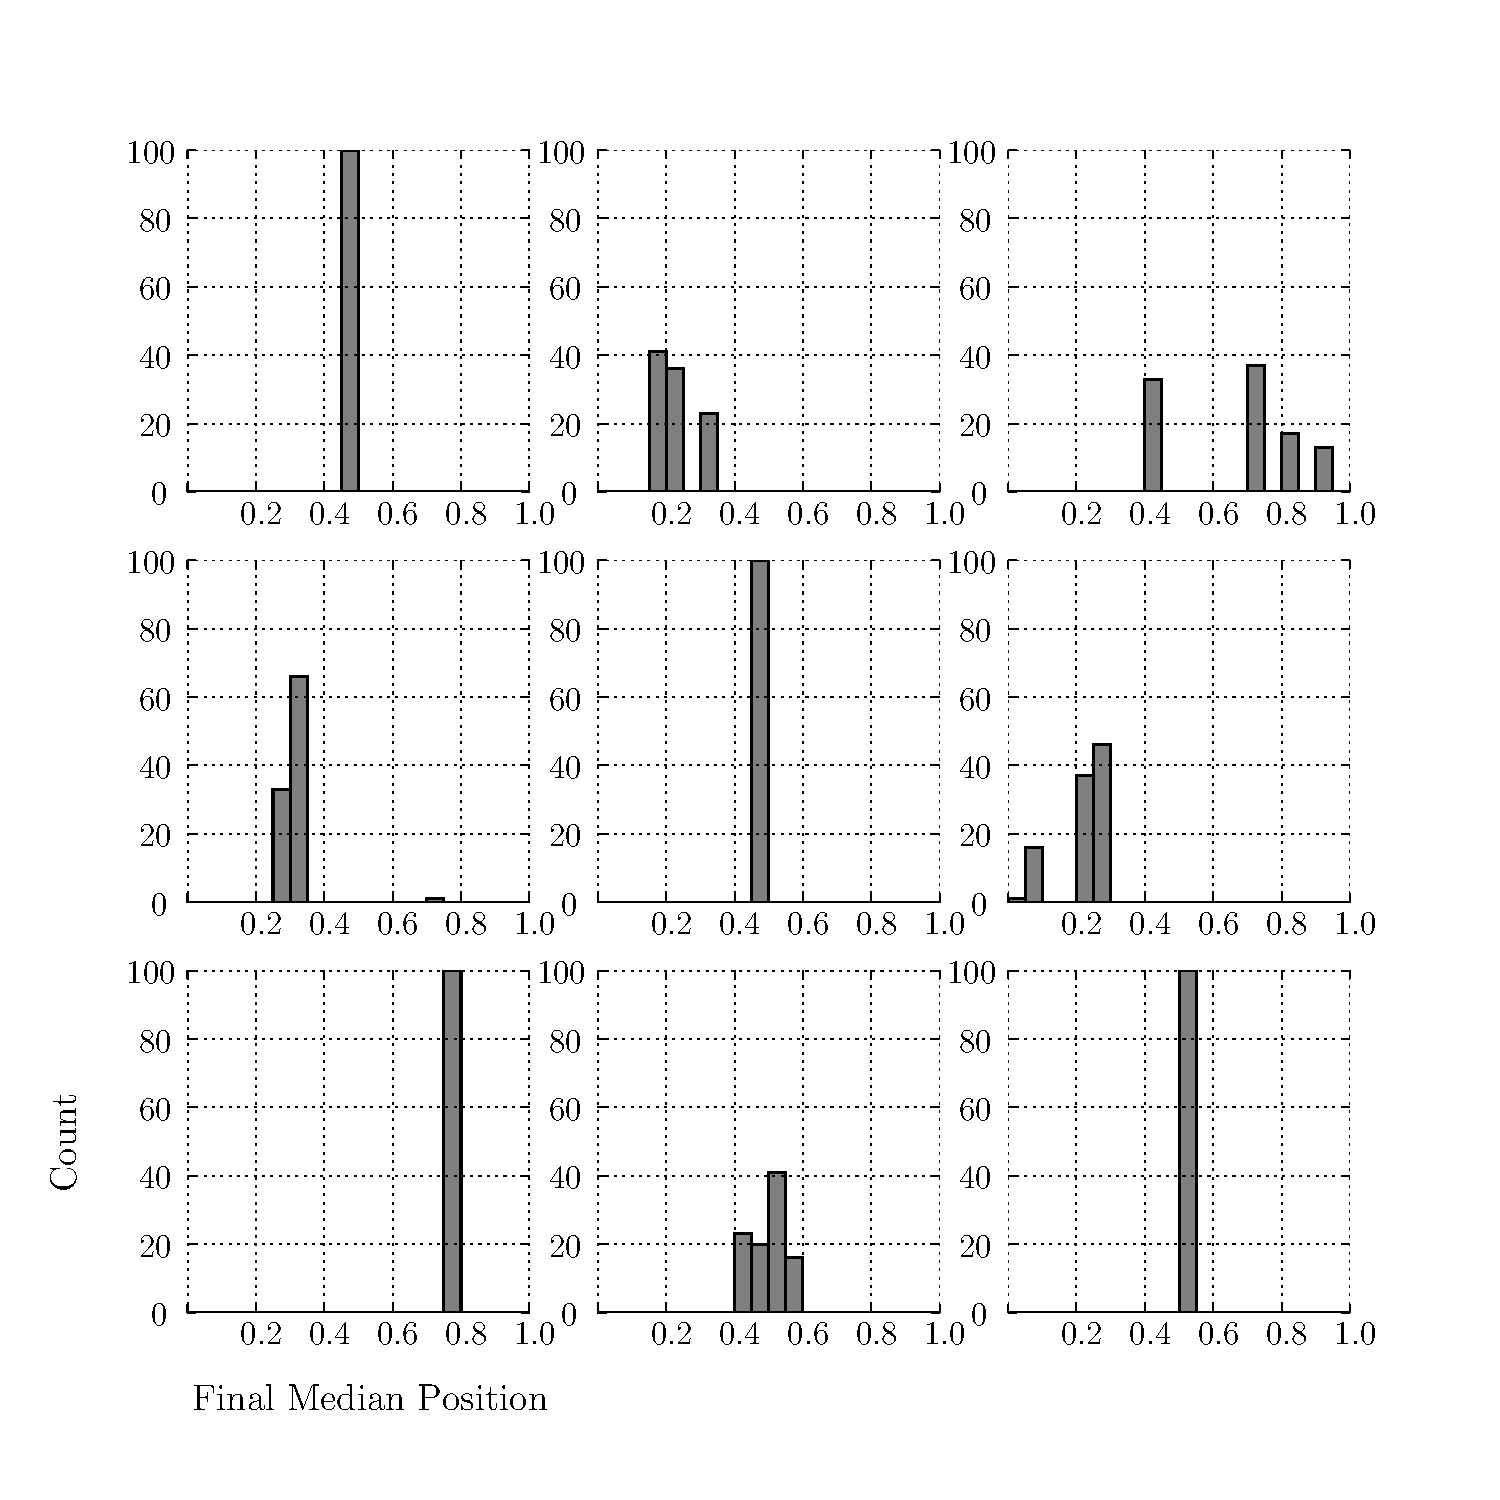
\includegraphics[width=\textwidth]{BDM_Reproduction/Figures/RandomGamesHist1}
        \caption{Experiment 1}
    \end{subfigure}
    \begin{subfigure}{0.49\textwidth}
        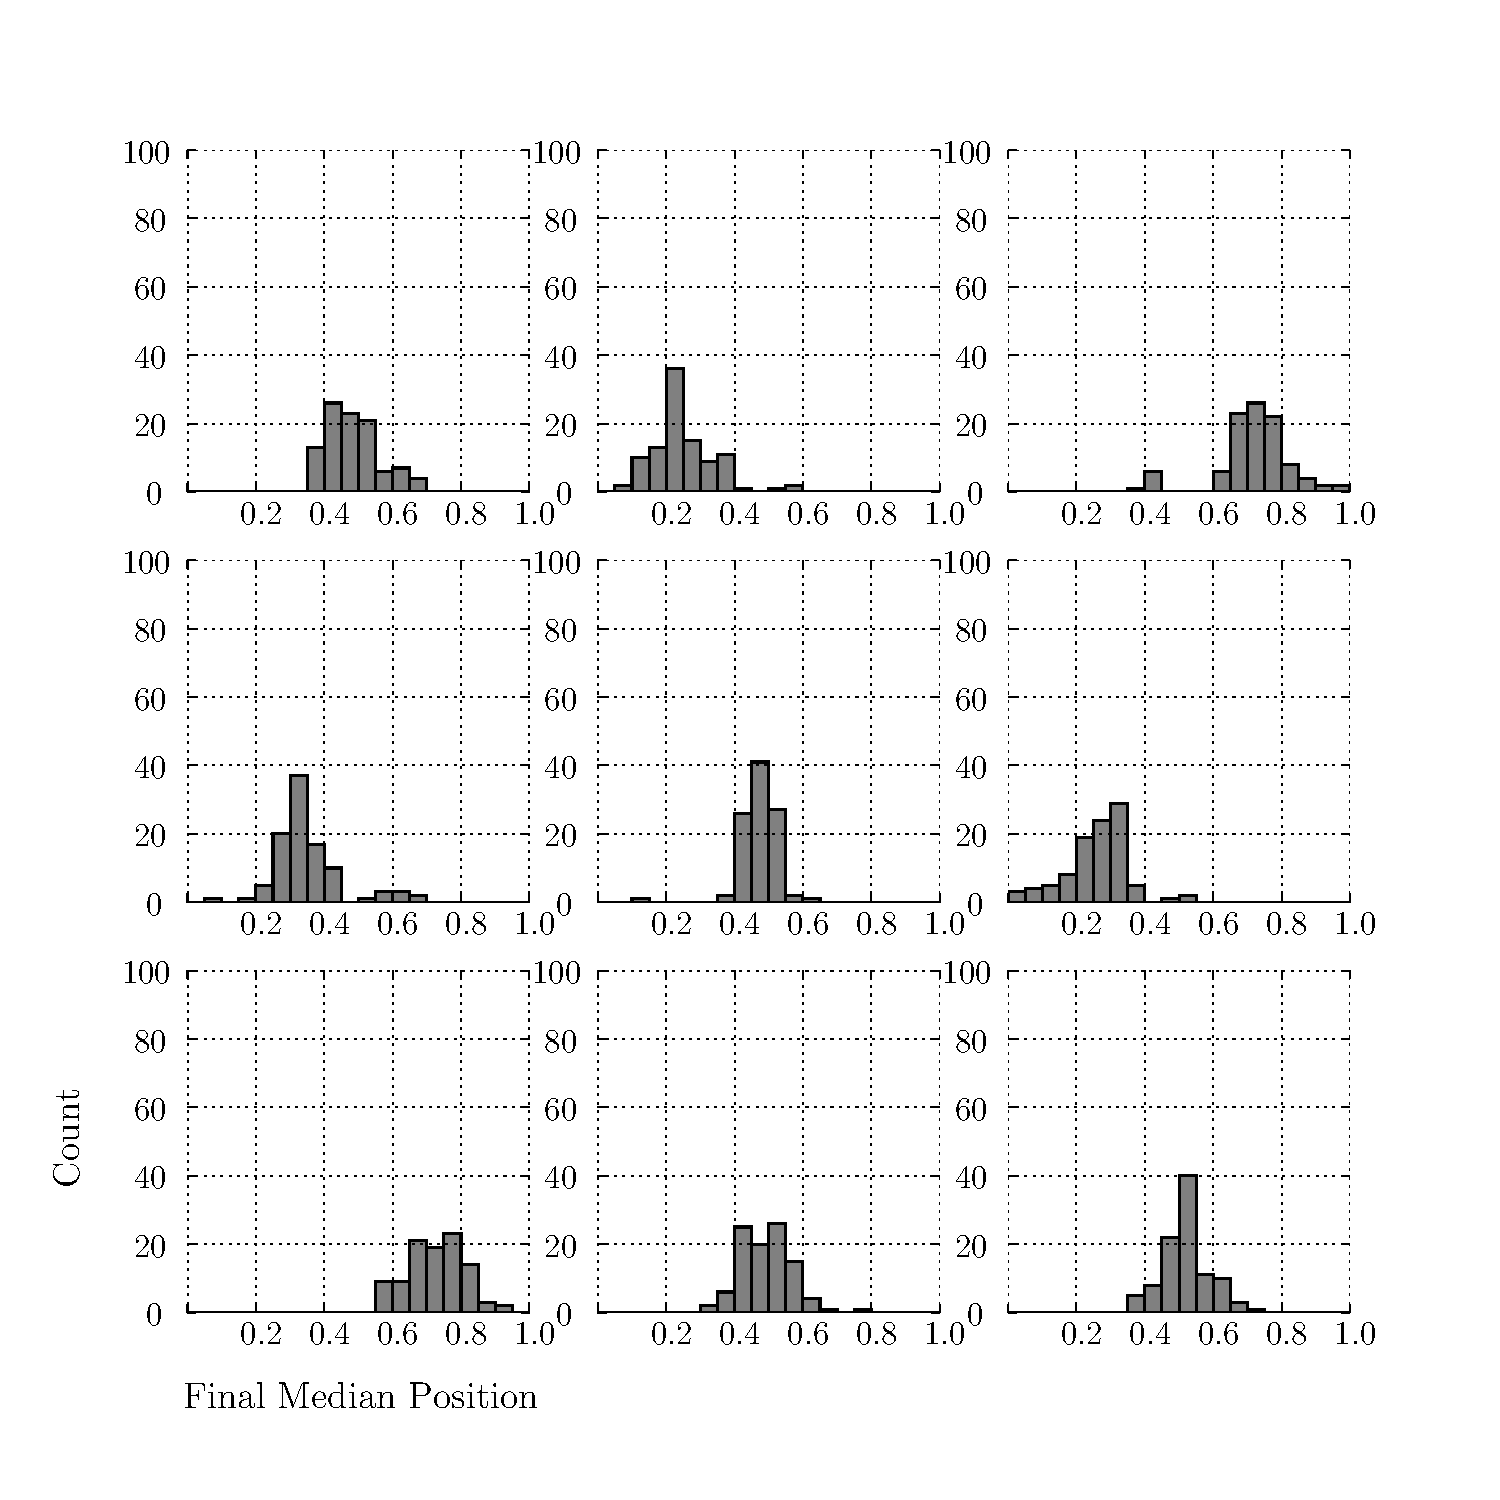
\includegraphics[width=\textwidth]{BDM_Reproduction/Figures/RandomGamesHist2}
        \caption{Experiment 2}
    \end{subfigure}

    \caption[Histograms of Median Positions]{Histograms of Median Positions from Nine Artificial Cases}
    \label{fig:random_medians}
    \figSpace
\end{figure}

Next, we can attempt to characterize the resulting distributions. Visual examination suggests that many of the resulting distributions are approximately normal. Applying the \citet{dagostino_1971} normality test to each dataset shows that only 25 of the cases generate normal distributions of outcomes in Experiment 1, while 43 do so in Experiment 2.

\begin{figure}
    \centering
    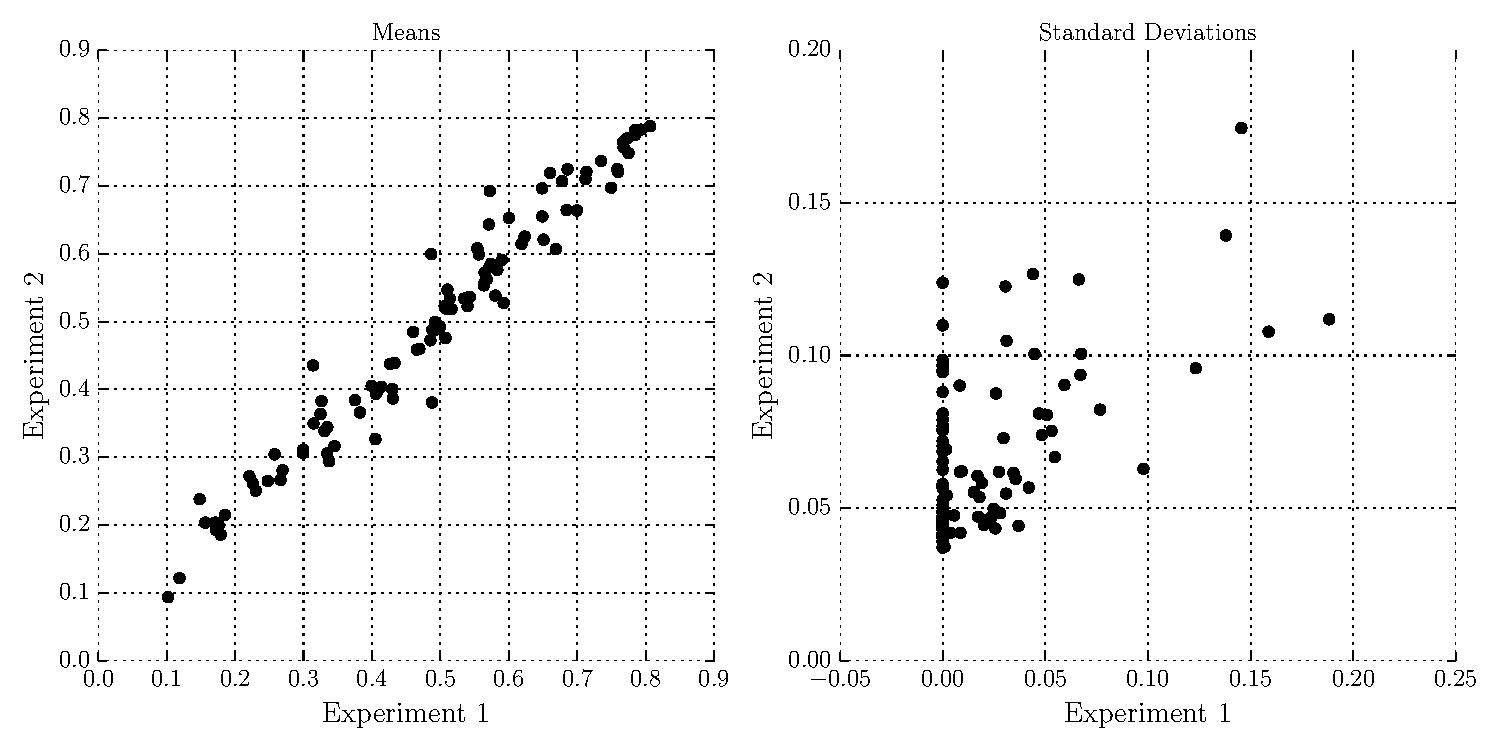
\includegraphics[width=\textwidth]{BDM_Reproduction/Figures/RandomGamesComparison}

    \caption{Experiment 1 and 2 Comparison}
    \label{fig:random_comparison}
    \figSpace
\end{figure}

Figure \ref{fig:random_comparison} compares the mean and standard deviation of outcomes from each case across both experiments. The key thing to observe is that the means of both are nearly identical. This means that though the perturbations of Experiment 2 increase the range of possible outcomes, they remain centered on the same outcome value; at no point does the perturbation appear to drive the model to a distribution qualitatively different from the non-perturbed outcomes. Additionally, the perturbation generally -- though not always -- increase the uncertainty of the model outcome, as measured by the outcomes' standard deviation. Furthermore, cases with similar degrees of uncertainty without perturbation (including no uncertainty, in the case of convergent cases) can yield different degrees of uncertainty once perturbed. 


\section{Information Extraction} \label{info_extraction}

At its most basic level, this model is meant to predict the outcome of the issue under negotiation. The outcome is generally defined as the median voter positions \citep{black_1948}: the position currently held by one of the actors which would defeat all other positions in bilateral contests. However, this may not be the most useful piece of information the model provides, particularly since many issues do not end up being resolved by a `vote,' or indeed resolved at all. In this section I will describe several additional outputs which can be extracted from the model, analyzed in their own right, and compared to empirical data.

One key piece of information the model generates is the set of the positions held by each actor at each iteration, and the trajectories of these positions. In cases where the position values represent concrete outcomes, the model provides a prediction (either a point prediction or a distribution) of the position each specific actor will hold. By examining how each actor's position changes, we can estimate the firmness of their position within the broader system being modeled. 

Furthermore, actor positions represent not just particular desired outcomes, but alignment with regard to other actors in a particular model run. If the model predicts two or more actors' positions moving together, we can interpret this as a prediction of cooperation, and potentially a formal or informal alliance, between these actors. Certainly, it is a prediction of convergent interests. This interpretation is shown in \citet{bdm_1998}, where certain model runs have agents' positions converging in ways that qualitatively resemble real-world alliances. This methodology can be formalized, by using the simulated distances between agent positions as a predictor for alliances or other relationships between the corresponding states. These distances can be used as an independent variable in several models, with alliances as the dependent variables: most simply a logistic regression, or network methods such as exponential random graph models (ERGMs) \citep{robins_2007} or latent space models \citep{hoff_2002}.

The model does not just generate positional predictions; each step generates discrete events from each interaction between a dyad of actors. While there is not have a clear mapping between model steps and real-world time, model-generated events can be compared to historic events within a window of interest; alternatively, the sequence of events can be compared, without taking into account the time-difference between them. Across multiple model instantiations, we can examine the frequency at which different events occur, either across an entire run or within a specified number of steps. 

The most obvious events, of course, are conflicts. Every model run may generate sets of conflict events when one or both of a pair of agents (depending on the model variant) choose to engage in conflict with each other. Conflict events are the most well-documented type of event in international relations, recorded in multiple specialized datasets \citep[e.g.][]{jones_1996,leng_1988,hendrix_2013} and are over-represented in media-coded event datasets \citep{schrodt_2001b}. This is particularly true when the conflict is overt between major political actors: military action is more likely to be recorded, while verbal conflict inside of a closed negotiation session less so.

Each conflict also creates a set of secondary events, with regard to the actors contributing capability to one side or another. The model does not specify what form this contribution takes; in reality, corresponding events may be positive actions towards the actor being supported (e.g. transfers of weapons or other materiel, favorable economic considerations), or negative actions towards the other side of the conflict (e.g. sanctions, withdrawal of support or access to resources). There may even be cooperative events observed between actors who are both supporting the same third party in its own conflict.

Offers are also events, though their correspondence with real events is also difficult to interpret. The model generates a much larger number of offers than end up being chosen, or even having a direct effect on the decisionmaking of the receivers. However, inasmuch as a conflict can only happen in the presence of threats, these threats may be treated as low-intensity conflict events as well.

\section{Comparing Model to Event Data} \label{icews}

The section above described how the model generates dyadic events, which can be compared to observed data. In this section, I describe implementing such an analysis in practice. I will walk through the instantiation of a set of geopolitical model runs using multiple different model variants, and comparing the conflicts they generate with observed micro-level event data in order to test and compare how well each explains the observed events. 

I set up several model variants, each using some different combinations of sub-models, based on different assumptions. I instantiate each with the same country-level agents with data from 2004, a year chosen arbitrarily for being well-covered by event data sets and lacking any major geopolitical shocks in the following years. I run each instantiation of the model for 24 steps, corresponding to approximately two years of `real' time. This mapping is somewhat arbitrary, but is based on the conventions which have developed for aggregating event data \citep{yonamine_2011}. In general, states do not change position or decide to begin or end confrontations with others on a day-by-day basis; however, neither do they do these things only once per year. Running these models multiple times produces a set of simulated events. I then run several tests to measure whether these simulated events are useful as predictors of real events. Comparing the predictive power of the model variants to one another can allow us to assess which variant is more predictive -- and thus, be provide evidence in support of their underlying assumptions.

\subsection{Data Sources} \label{data_sources}

\subsubsection{Event Data}

Real-world event data will serve as the dependent variable we are attempting to predict. The event data source I use for this is the Integrated Crisis Early Warning System, or ICEWS. This is a dataset of international political events, and specifically actions, extracted and machine-coded from media sources \citep{boschee_2015}. Each event consists of a Source (who carried out the action), a Target (who the action was directed at), and a code for the action itself. Actors (sources and targets) are coded to country, sector (e.g. government, civilians, rebels) and when possible to unique entities. Actions are assigned an Intensity score, where positive and negative values are associated with positive and negative actions, respectively. ICEWS has been assessed as being the most complete and reliable of several similar event datasets currently available \citep{ward_2013b}; however, on principle this analysis could be conducted with other event datasets as well.

In order to extract events which can be directly compared to model output, I subset the data and select events meeting the following criteria:

\begin{itemize}
    \item Occurring in the years 2005-2006, so that they are strictly following the input data.
    \item Where both the Source and Target actors are coded with the Government sector. This excludes events involving civilians, rebels, and other actors not explicitly captured in the model.
    \item Where the Source and Target countries are different, excluding internal events.
\end{itemize}

With these criteria, I aggregate the events into counts of event type by directed dyad. For the purposes of this analysis, I am not looking at the ordering of these events with respect to one another, but merely that they occur. 

\subsubsection{Input Data}

Following the methodology in \citet{bdm_1998}, I set agent properties based on the Correlates of War (COW) dataset: specifically, the alliance \citep{gibler_2004} and national material capabilities (NMC) \citep{singer_1988,grieg_2010} datasets. 

Using the material capabilities dataset, I select the 50 states with the highest Composite Index of National Capability scores. These are the model agents, and their CINC values are used as their capabilities. Since capabilities are always used in the model to compute ratios, there is no need to normalize these scores any further. Salience values will be set randomly, as described below.

Next, I use the COW alliance data to estimate positions. Taking advantage of the so-called unipolarity of the international system \citep{wohlforth_1999}, I will set each actor's initial position as the similarity of its alliance portfolio to that of the United States. Similarity of alliance portfolio has been used an approximation of the alignment of two countries' interests \citep{bdm_1975}, and alignment with the system's most powerful actor serves as a rough estimate of geopolitical position. 

Using  the alliances in effect in the selected instantiation year of 2004, I assemble an undirected network of state-to-state relationships, with the relationship coding as the weight\footnote{Note that this network includes all the actors present in the COW data, not just the top 50 actors who will be included in the model: as we are using the network to estimate similarity of positions, even countries which are not powerful enough to be worth including as agents can serve as indicators of countries' interests, and thus worthwhile to include in the network}. Using the resulting network's adjacency matrix, I compute the tau-b similarity \citep{bdm_1975} between country rows, and specifically between each country's row and that of the United States.

%
%\begin{figure}
%  \centering
%  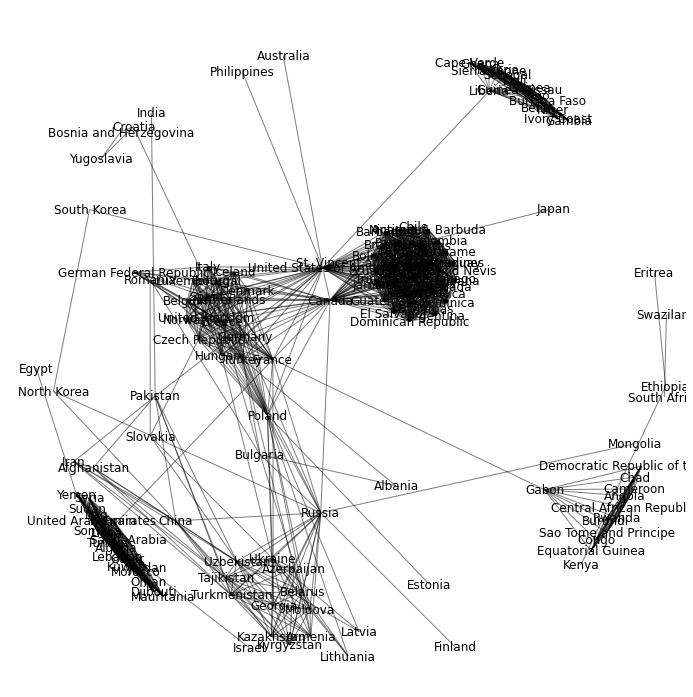
\includegraphics[scale=0.5]{BDM_Reproduction/Figures/Alliances2004}
%  \caption{Alliance network in 2004}
%  \label{fig:alliances_2004}
%  \figSpace
%\end{figure}
%
%\subsection{Model Setup}

Using the NMC and estimated positional data, I instantiate a model with 50 agents, one per state. There are 8 states which do not appear in the alliance network; at the beginning of each instantiation, I arbitrarily assign each a position of 0.5 + $\epsilon$, where $\epsilon \sim Normal(0, 0.1)$. The random perturbation is in order to prevent them from becoming a single alliance bloc. 

\begin{table}[h!]
\centering
\caption{Model Parameters}
\label{table:model_parameters}
\begin{tabular}{cl}
    \hline
    Variable &  Value \\
    \hline
    $s_i$            &        $\sim Unif(0, 1)$          \\
    $Q_i$            &   $0.5$ \\
    $T_i$            &   $0.5$ \\
    \hline
    Number of steps per run &        $24$ \\
    Number of instantiations &        $100$ \\
    \hline
\end{tabular}
\tableSpace
\end{table}

Unlike position and capability, there is no dataset giving us a-priori information on the agents' salience, particularly when the issue is relatively broad, as it is here. Thus, I apply salience updating rule $\mathbf{S_2}$: for each model instantiation, I set all the agents' saliences randomly, such that $s_i \sim Unif(0,1)$. As it is unlikely that shocks changing agents' salience will occur on a monthly basis, I hold these saliences constant throughout all 24 steps; this simplifying assumption removes one source of noise. This also corresponds to the assumption in \citet{bdm_1998} (which is also used in the following chapter), whereby agents' saliences are re-randomized on timesteps corresponding to approximately two years.


\begin{landscape}
\begin{table}
\centering
    \caption{Agent Data}
    \label{table:icews_agent_data}
\begin{tabular}{lcc|lcc}
    \hline
        Name                             & Position & Capability & Name                     & Position & Capability \\
    Algeria                          & 0.007    & 0.005      & Mexico                   & 0.734    & 0.012      \\
    Argentina                        & 0.732    & 0.005      & Morocco                  & 0.007    & 0.004      \\
    Australia                        & 0.192    & 0.007      & Myanmar                  & --      & 0.007      \\
    Bangladesh                       & --       & 0.008      & Netherlands              & 0.548    & 0.006      \\
    Belgium                          & 0.548    & 0.005      & Nigeria                  & 0.059    & 0.007      \\
    Brazil                           & 0.734    & 0.024      & North Korea              & 0.229    & 0.013      \\
    Canada                           & 0.907    & 0.011      & Pakistan                 & 0.092    & 0.013      \\
    Chile                            & 0.732    & 0.003      & Philippines              & 0.192    & 0.006      \\
    China                            & 0.115    & 0.183      & Poland                   & 0.45     & 0.007      \\
    Colombia                         & 0.734    & 0.006      & Romania                  & 0.271    & 0.004      \\
    Democratic Republic of the Congo & 0.072    & 0.004      & Russia                   & 0.141    & 0.045      \\
    Egypt                            & 0.192    & 0.009      & Saudi Arabia             & 0.007    & 0.009      \\
    Ethiopia                         & 0.17     & 0.004      & South Africa             & 0.192    & 0.007      \\
    France                           & 0.485    & 0.02       & South Korea              & 0.17     & 0.024      \\
    Germany                          & 0.55     & 0.027      & Spain                    & 0.548    & 0.011      \\
    Greece                           & 0.514    & 0.004      & Sweden                   & --       & 0.005      \\
    India                            & 0.324    & 0.07       & Syria                    & 0.008    & 0.004      \\
    Indonesia                        & --       & 0.013      & Taiwan                   & --       & 0.008      \\
    Iran                             & 0.168    & 0.012      & Thailand                 & --       & 0.008      \\
    Iraq                             & 0.007    & 0.006      & Turkey                   & 0.475    & 0.014      \\
    Israel                           & 0.192    & 0.004      & Ukraine                  & 0.088    & 0.014      \\
    Italy                            & 0.548    & 0.019      & United Kingdom           & 0.548    & 0.021      \\
    Japan                            & 0.192    & 0.047      & United States of America & 1        & 0.143      \\
    Kazakhstan                       & 0.056    & 0.003      & Venezuela                & 0.734    & 0.005      \\
    Malaysia                         & --      & 0.004      & Vietnam                  & --      & 0.008     \\
    
    \hline
\end{tabular}
\tableSpace
\end{table}

\end{landscape}


\subsection{Model Variants}

There are multiple possible permutations of the various sub-model variants presented in Sections \ref{model_description}. In this section, I will test a subset of them, attempting to cover a range of possible differences. In light of the coercion question I discuss in \ref{conflict_coercion}, I vary the conflict sub-models $\mathbf{W_0}$ and $\mathbf{W_1}$ across several variants. Recall that $\mathbf{W_0}$ has the loser in each conflict adopt the winner's position, while in $\mathbf{W_1}$ conflicts lead neither actor to change position.

\begin{description}
    \item[Model 1a]: This is the attempted replication of the original BDM model, as described in detail in Section \ref{model_description}. It comprises the sub-models  $\{\mathbf{T_0, S_2, W_0, R_0, O_0, M_0, A_0}\}$
    \item[Model 1b]: This model variant is identical to the one above except for the conflict sub-model. This variant will test the hypothesis that removing explicit coercion would make the model better reflect reality, and hence improve its explanatory and predictive power. $\{\mathbf{T_0, S_2, W_1, R_0, O_0, M_0, A_0}\}$
    \item[Model 2a]: This model implements several of the model variants together, while adhering to the overall structure of the original. Importantly, it implements the modified conflict schedule, with conflicts occurring only after agents have changed position in response to offers. $\{\mathbf{T_1, S_2, W_0, R_1, O_0, M_1, A_0}\}$
    \item[Model 2b]: Similarly, this model implements the previously-discussed variants, changing the conflict model. $\{\mathbf{T_1, S_2, W_1, R_1, O_0, M_1, A_0}\}$
    \item[Model 3a]: This model variant is the most different from the baseline. In addition to the new schedule and risk sub-models, it implements the balancing and attack follow-through sub-models. Unlike the other model variants here which require both agents in a conflict to choose to enter into it, this variant allows for unilateral attacks. $\{\mathbf{T_1, S_2, W_0, R_1, O_0, M_2, A_1}\}$
    \item[Model 3b]: Finally, once again, this variant is identical to the previous one, but uses the alternative conflict sub-model. $\{\mathbf{T_1, S_2, W_1, R_1, O_0, M_2, A_1}\}$
\end{description}

\subsection{Experiments and Results}

For each model variant, I instantiate 100 model runs with the data in Table \ref{table:icews_agent_data}. I then run each for 24 steps. For each model run, I extract the Conflict events that the model generates. I aggregate these events across all runs for each dyad, and compute the mean conflict events for each dyad. These mean conflicts are the independent variables. 

\begin{figure}[t!]
    \centering
    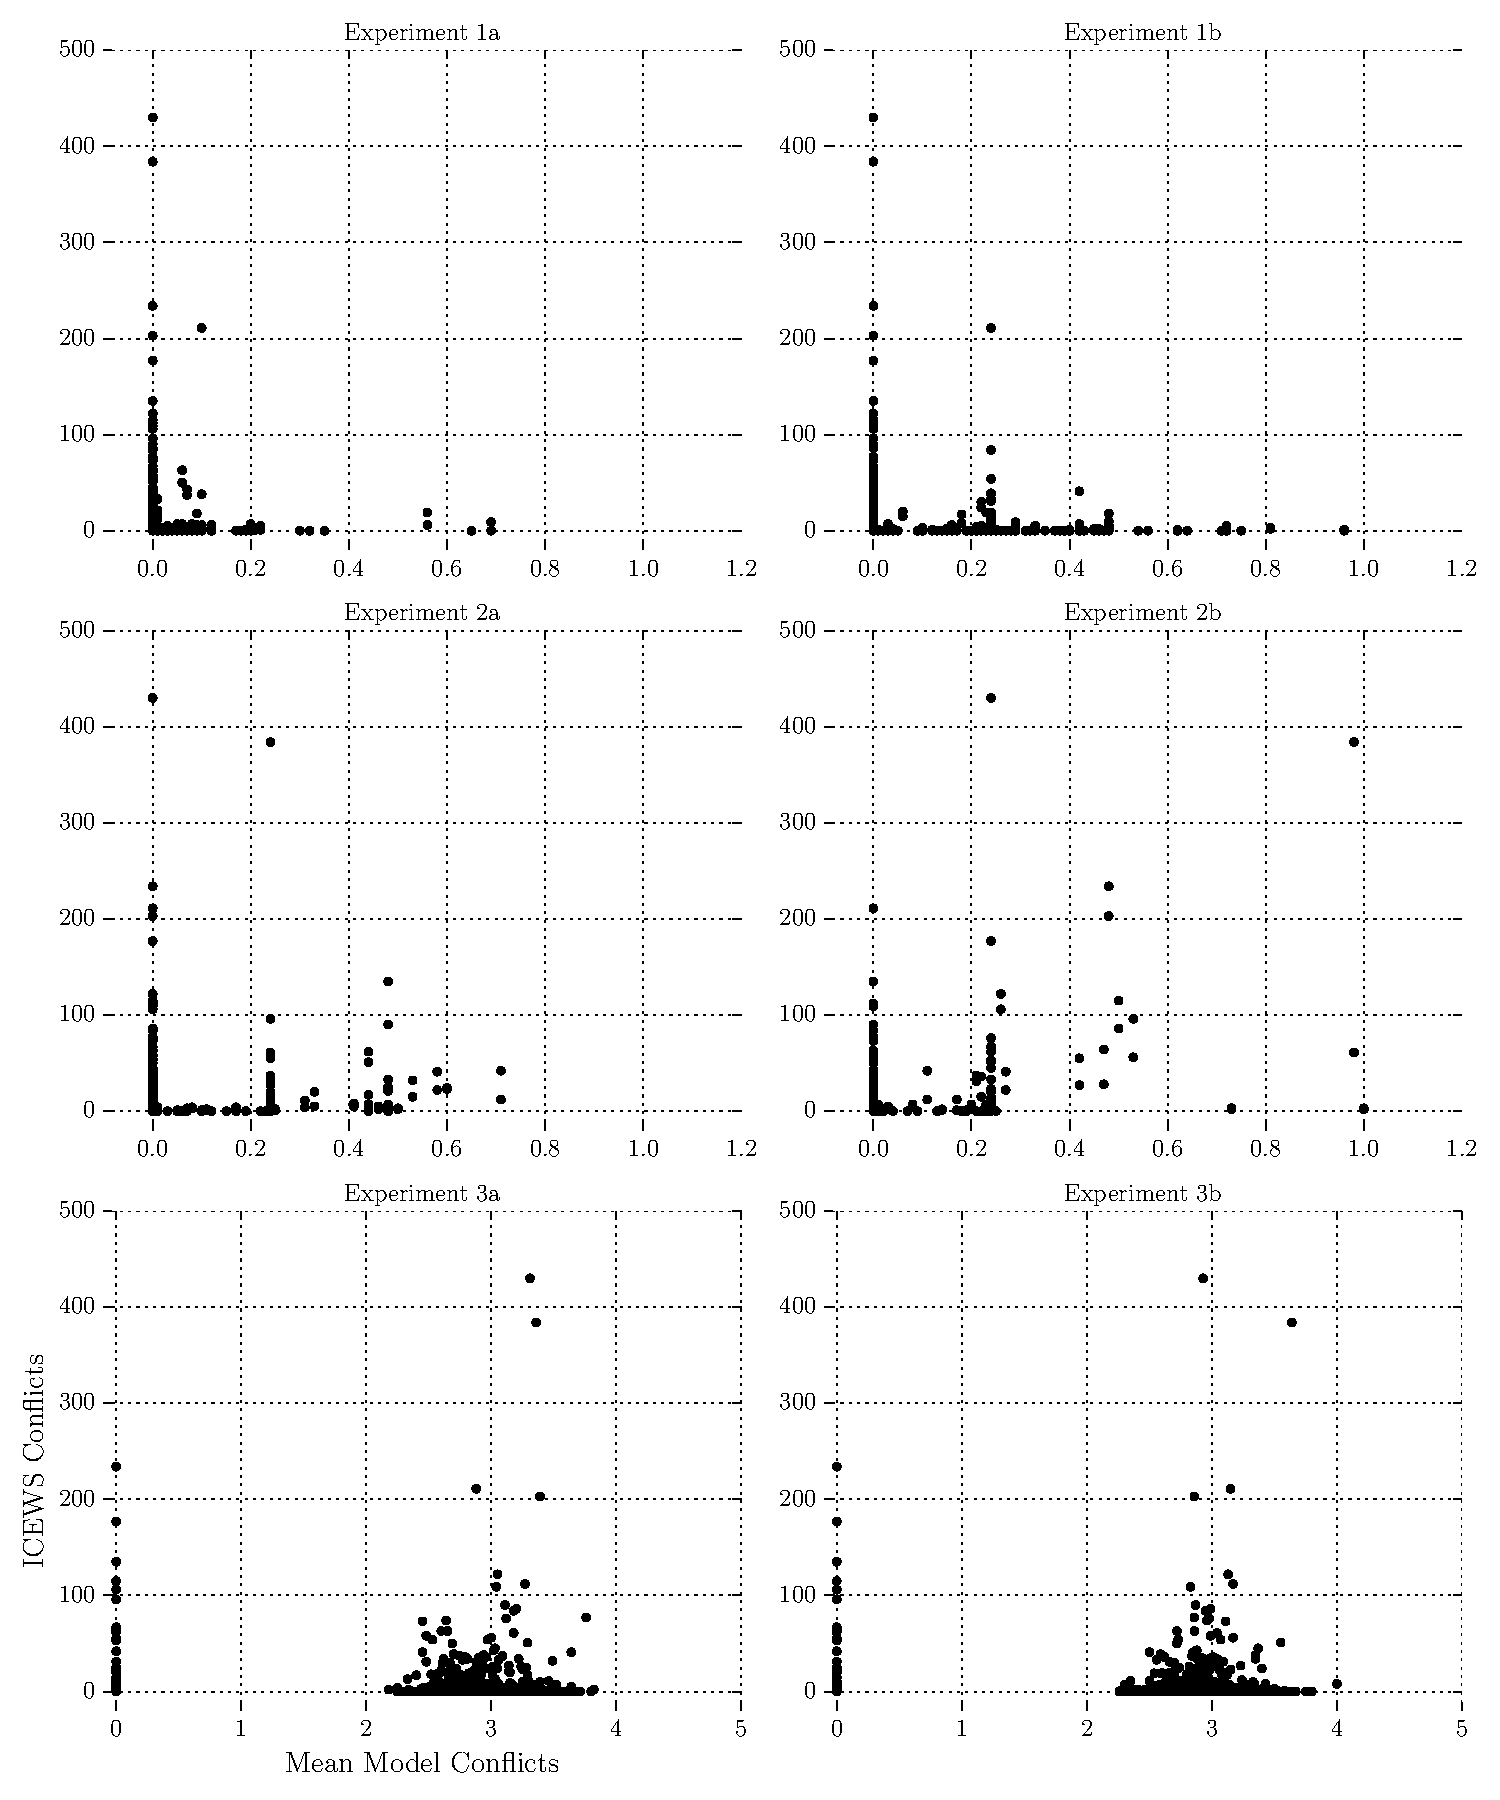
\includegraphics[width=\textwidth]{BDM_Reproduction/Figures/ICEWS_Scatters}
    \caption{Model-Generated vs ICEWS Conflict Events}
    \label{fig:icews_scatters}
    \figSpace
\end{figure}

The dependent variables are the conflict-coded events for each dyad drawn from the ICEWS dataset for the 2005-06 period, as described above in Section \ref{data_sources}. Figure \ref{fig:icews_scatters} shows the scatter-plots of total model-generated conflicts versus ICEWS conflict events for each dyad. It is immediately obvious that a large portion of these two result sets are orthogonal: many dyads with ICEWS conflicts do not have model conflicts, and vice versa.  I next test whether, for each model variant, the simulated events it generates have any predictive power for the volume of conflict events predicted for each dyad. I conduct two sets of regressions, on two variables: a linear model on the number of observed conflict events (Table \ref{table:icews_linear}), and a logistic regression on whether any conflicts were observed across each dyad (Table \ref{table:icews_logit}). In both cases, the mean model-generated conflicts are be the independent variable. 

These are relatively simple statistical models; in particular, we have no reason to expect there to be a linear relationship between simulated and observed conflicts. However, these regressions will allow us to identify whether a relationship exists at all between the simulated and observed events, and what direction that relationship is -- in general, we expect that if a model is generating plausible conflicts, there will be a positive relationship between simulated and observed conflict events. Furthermore, since the dependent data is the same across all model variants, we can directly compare the coefficients and fit to determine which model is closer to reality.


\begin{table}

\begin{center}
    \caption{ICEWS Conflict Events -- Linear Regressions}
    \label{table:icews_linear}
\begin{tabular}{lcccccc}
    \hline
                    &    1a   &    1b    &    2a    &    2b    &    3a    &    3b     \\
    \hline

    Const.          & 2.82*** & 3.91***  & 2.27***  & 1.40***  & 20.37*** & 21.80***  \\
                    & (0.35)  & (0.44)   & (0.35)   & (0.33)   & (2.10)   & (2.10)    \\
    Mean Model Conflicts & 6.82    & -7.90*** & 33.58*** & 94.31*** & -6.20*** & -6.64***  \\
                    & (8.61)  & (1.99)   & (4.57)   & (4.38)   & (0.73)   & (0.73)    \\
    \hline
    $R^2$             & 0.00    & 0.01     & 0.02     & 0.16     & 0.03     & 0.03      \\
    \hline
    \hline
    \multicolumn{7}{l}{Standard errors in parentheses.} \\
    \multicolumn{7}{l}{* $p<.1$, ** $p<.05$, *** $p<.01$} \\

    \end{tabular}
    \end{center}
    \tableSpace
\end{table}

\begin{table}
\begin{center}
    \caption{ICEWS Conflict Events -- Logistic Regressions}
    \label{table:icews_logit}
\begin{tabular}{lcccccc}
    \hline
                    &    1a   &    1b    &    2a    &    2b    &    3a    &    3b     \\
    \hline
    Const.          & -1.19*** & -1.03*** & -1.30*** & -1.32*** & 1.22***  & 1.47***   \\
                    & (0.05)   & (0.06)   & (0.05)   & (0.05)   & (0.30)   & (0.31)    \\
    Mean Model Conflicts & 2.27**   & -1.15*** & 5.52***  & 8.01***  & -0.86*** & -0.94***  \\
                    & (1.03)   & (0.30)   & (0.62)   & (0.81)   & (0.10)   & (0.11)    \\
    \hline
    Pseudo $R^2$      & 0.00     & 0.01     & 0.03     & 0.05     & 0.03     & 0.04      \\
    \hline
    \hline
    \multicolumn{7}{l}{Standard errors in parentheses.} \\
    \multicolumn{7}{l}{* $p<.1$, ** $p<.05$, *** $p<.01$} \\
    \end{tabular}
    \end{center}
\tableSpace
\end{table}

Examining Table \ref{table:icews_linear} immediately shows us that there are substantial differences between the predictive power of the different models. The output of Model 1a, the original model, seems to bear no measurable relationship to the observed events. Models 1b, 3a and 3b have negative mean conflict coefficients, indicating that the more simulated conflicts we observe, the fewer real conflicts we can expect to see -- the opposite of the relationship we were hoping for. Only Models 2a and 2b have coefficients which are significant and positive, showing that the more conflicts these models predict, the more we can expect to see. Between these two, Model 2b has a substantially higher $R^2$ value, indicating a better fit. 

The same pattern holds when examining Table \ref{table:icews_logit}, which coarse-grains the ICEWS data further, asking whether more simulated conflicts make it more likely that we will observe any conflicts at all between the corresponding dyad. The coefficients show the same pattern of signs, indicating that only Models 2a and 2b generate simulated conflicts which are useful for predicting real conflicts. Between these, again, Model 2b shows a better fit, though the advantage is less stark here.

%In order to further test whether these models are providing useful new information, I repeat the regressions above, with an additional variable: the tau score for each dyad, or the estimated similarity of the two actors' interests to one another. Based on theory, we would expect more observed conflict events between actors with lower tau scores. The results of these regressions are shown in TKTKT. Two results jump out: first is that the coefficients on tau are positive, indicating more conflict events the more similar two actors are -- a surprising deviation from theory worth exploring in more detail, but outside the scope of this paper. More importantly, for our purposes, the \textbf{Model Conflicts} coefficients both remain small but positive, with only the baseline variant remaining statistically significant. This indicates that the baseline model, at least, is indeed generating new information rather than simply arriving at the same result as the tau-based analysis via a circuitous route. 

\subsection{Discussion}

With these results in hand, we can draw several conclusions. At the crudest level, we see that across all the model variants, the number of conflict events generated is much smaller than the number of observed conflict events. Many dyads with recorded conflict events are not predicted by the models, while the models in turn predict conflicts across many dyads where none are observed. The overall relationships between the model outputs and observed data are weak.

Despite this, we must recall that there are countless issues that at any given time are driving the micro-level interactions between countries in the world. Across all the model variants presented here, we have attempted to capture only those issues reflected in states' alliances, and further compressed them onto a single one-dimensional space. Given the simplicity of the model itself, and the global scope that these particular instantiations are addressing, and it appears remarkable that there is any statistical relationship between the model output and reality at all. And indeed, several of the model variants -- particularly 2a and 2b -- appear to be valid, if weak, predictors of real-world conflicts, at least as captured by the ICEWS data.

Furthermore, this methodology allows direct comparison between model variants, each comprising combinations of different sub-models. Examination of the scatter-plots of Figure \ref{fig:icews_scatters} shows us that different variants generate different patterns of events. We can immediately see, in particular, that Models 3a and 3b generate a higher volume of conflict events, and that the quantities for each dyad are approximately normally-distributed, conditional on there being any conflicts at all for those dyads. We can also immediately identify that variants 2a and 2b outperform the other variants as predictors, and that between the two of them variant 2b has superior predictive power. This, in turn, is in line with my hypothesis that the conflict sub-model $\mathbf{W_1}$, where conflicts do not result in agents changing their position, is will capture the underlying system better than the baseline variant $\mathbf{W_0}$.

\section{Conclusions}

In this chapter, I have argued that Bruce Bueno de Mesquita's Expected Utility Model is best understood not as a game-theoretic model but as an agent-based one. The model and its agents are composed of several sub-models, with the agents interacting with one another following certain behavior rules. These rules, in turn, are based on heuristics and embedded assumptions, many of which are not addressed in prior papers describing the model and its applications. I have described my reimplementation of the model as an object-oriented agent-based model. While doing so, I was able to identify its sub-models and heuristics, and discuss how they fit together -- and how they may be altered and experimented with.

My reimplementation of the model was unable to reproduce several results generated by the original model and reported in the prior literature, in particular the results of \citet{bdm_1994} and \citet[chapter 6]{bdm_2002}. It is possible that despite my best efforts, my own model code misimplements one of the formulas from the prior literature, or has another unidentified bug which is the cause of the difference between its outputs and the prior results. It is also possible that I have implemented one of the sub-models which is not well described in the prior literature (particularly the offer acceptance sub-model) differently from the original model. Without access to the original application or source code, it is impossible to fully isolate the source of the differences. Nevertheless, I do have access to the source code of the \citet{scholz_2011} model implementation, as well as to a replication of that implementation \citep{mckibben_sanders_2014}, both of which successfully reproduce the \citet{bdm_1994} results. As I discuss in Section \ref{verification}, I identify a key way in which this implementation contradicts both the stated form and underlying assumptions of the original model, by having the probabilities of victory in a bilateral conflict not sum to 1. It may be the case that by coincidence this model implementation featured multiple errors which lined up to produce the right results for the wrong reasons; however, as \citet{scholz_2011} themselves note, the odds of generating correct results by chance are extremely low. It seems more likely that they have inadvertently identified an error in a particular implementation of the original model -- one which, presumably, was corrected in later versions. Importantly, the \citet{scholz_2011} implementation was unable to replicate results reported in other publications. This tells us that their implementation cannot be considered a perfect replication either -- and that published original model results cannot necessarily be treated as `ground truth' either.

In Section \ref{sensitivity-analysis}, I described and implemented a sensitivity analysis methodology using randomly generated cases. This analysis indicates that the original model has little meaningful stochasticity, and that in many cases converges to a single median outcome. In fact, it suggests that there are two distinct classes of input sets, those which have deterministic outcomes and those that do not. This distinction should be investigated further, in particular in applications of the model to the analysis of real-world cases. Even relatively slight perturbation of the model inputs introduced an additional source of stochasticity, eliminating the determinism. It also does not appear to be the case that convergent models have less uncertainty once the inputs are perturbed, suggesting that the convergence is an artifact of the specific input parameters rather than evidence that the system itself has an inherent attractor. However, the means of the perturbed runs tend to remain very close to the unperturbed mean; the perturbation doesn't push the system into a meaningfully different region of the outcome range. This finding, in turn, lends justification to practice of original model results being reported as point predictions rather than distributions.

The model itself is driven largely by heuristics, with the model and agent behavior not always grounded in specific theories or sources. This on its own is not necessarily a major flaw, and indeed is common for other agent-based models of international relations \citep[e.g.][]{axelrod_1997,taylor_2008}. By reimplementing the model as an ABM, I was able to highlight these heuristics and assumptions to a greater extent than had been previously reported. More importantly, this implementation makes it straightforward to test the model with different sub-models and heuristics reflecting different assumptions. I have proposed several such variant sub-models, as well as a notation system to quickly describe different model variants comprising different sub-models.

By enabling multiple model variants to be run with the same input data, I also test the predictive power of those variants side by side. Political event data provides a source of relevant real-world interactions, and to the best of my knowledge, no EUM-type model has been applied to event data before. However, as I argue in Section \ref{info_extraction}, the dynamics and outputs of the model correspond naturally to categories present in event data. Indeed, I demonstrate in Section \ref{icews} that even using a coarse instantiation without a well-defined issue of contention, several variants of the model generate sets of simulated events bearing weak but statistically significant predictive power for corresponding real-world events. 

More important than the specific findings of these models, however, is a demonstration of how such models can be applied comparatively. By using fixed input data and the same target output data, we can run multiple instantiations of different model variants, generating sets of model traces -- and especially sets of simulated conflict events -- for each. This allows us to find the different patterns which emerge from different models, such as the difference in conflict distributions between model variants 1, 2 and 3 visible in Figure \ref{fig:icews_scatters}. By regressing the model outputs against observed data, we can test which among several models has more explanatory or predictive power. Comparing the performance of model variants which differ only by a single sub-model (such as 3a and 3b above, which implement conflict rules $\mathbf{W_0}$ and $\mathbf{W_1}$, respectively) can highlight the effects of those sub-model variants, and allow us to test the hypotheses they describe.

The model and methodology I have described here mark the beginning, not the end, of a program of study. I have explored only a subset of possible combinations of the sub-models I have presented here, which in turn are only a subset of plausible sub-model variants. Applying the sensitivity analysis to additional model variants will allow us to characterize inherent dynamics or artifacts that the variants exhibit, which in turn can help isolate meaningful predictions when instantiated with real data. Testing these models against different cases and sets of political actors will help identify whether one mode variant is strictly superior, or whether different variants are appropriate for different categories of cases and issues. It may also be the case that ensembles of model variants may provide greater predictive power than any single variant alone. 

There are still assumptions embedded in the current architecture, independent of any sub-model. For example, conflicts are currently strictly bilateral, and agents contributing capability to one side or another face no effects if the principals win or lose, unlike in the \citet{wise_2015a} model framework. Similarly, the model as presented here only models issues as one-dimensional ranges; however, \citet{wise_2015b} have proposed an extension allowing their model to handle multiple issues, including ones represented non-numerically. The agent activation regime plays an important role in the behavior of agent-based models \citep{comer_2014}, and the validity of the simultaneous activation assumption may depend on the specifics of the scenario being simulated. The simultaneous activation the model currently features may be appropriate for modeling negotiators in close proximity (perhaps in the proverbial smoke-filled room) or when the actors are states acting over months or years, but may be less so for intermediate scales. Varying and sequencing agent activation may allow the model to incorporate time more explicitly, improve modeling of interactions between agents with different paces of decisionmaking, and endogenize incomplete information. 

There are likely other methods of utilizing models within the framework described here. I have conducted preliminary experiments with applying the model deductively: given observed sequences of events, to identify initial inputs which are most likely to give rise to similar sequences. This may allow us to estimate the actors' underlying preferences and capabilities in the absence of reliable quantitative data or even subject-matter expertise. My initial experiments suggest that such an application is computationally plausible, but that multiple, substantially different inputs may yield similar event sequences.

Finally, the findings I have described here provide reasons for both appreciation and skepticism of the original BDM model. Building on the published descriptions of the model have allowed me to build a generalized, flexible agent-based model of political interaction with rich outputs and surprising predictive power despite its relative simplicity. The sensitivity analyses I have conducted lend some credence to the practice of reporting the model's point results, though also highlight the degree to which this elides uncertainty that is indeed present in the model. The difficulty in reproducing the model from published descriptions should give us pause. I have identified numerous assumptions and heuristics in the model description, very few of which are explicitly stated, much less supported either theoretically or empirically. This makes it all the more important to implement not just a single model but multiple variants, in order to rigorously test and evaluate them. If we do so, however, it promises to offer a valuable tool for operationalizing and testing competing heuristics, intuitions and theories of competing political actors in the international system and beyond.
